% gjilguid2e.tex
% V2.0 released 1998 December 18
% V2.1 released 2003 October 7 -- Gregor Hutton, updated the web address for the style files.

\documentclass{gji}
\usepackage{timet}
\usepackage{amsmath}
\usepackage{graphicx}


\graphicspath{{./paper_figures/publishable/}}



\title[Comparisons of surface wave amplitude decay]
  {Comparisons of surface wave amplitude decay \\for colocated rotation and translation measurements}
\author[Bryant Chow]
  {Bryant Chow,$^1$\thanks{Now at Victoria University of Wellington, School of Geography, Environment and Earth Sciences, Kelburn Parade, Wellington, New Zealand 6012} 
  Heiner Igel,$^1$ 
  Joachim Wassermann,$^1$
  Bernhard Schuberth,$^1$  \vspace{2mm}\\
  \LARGE{{\normalfont C\' eline Hadziiannou,$^{1,2}$ and
  Stefanie Donner$^{1,3}$}}\vspace{2mm}\\
  $^1$ Department of Earth and Environmental Sciences, Ludwig-Maximilians-University Munich, Theresienstra\ss e 41, D-80333 Munich, Germany.\\
  $^2$ Department of Earth Science, University of Hamburg, Bundesstra\ss e 55, D-20146 Hamburg, Germany\\
  $^3$ Federal Institute for Geosciences and Natural Resources, Stilleweg 2, D-30655 Hannover, Germany \\E-mail: bryant.chow@vuw.ac.nz
  }
\date{}
\pagerange{\pageref{firstpage}--\pageref{lastpage}}
\volume{}
\pubyear{}

%\def\LaTeX{L\kern-.36em\raise.3ex\hbox{{\small A}}\kern-.15em
%    T\kern-.1667em\lower.7ex\hbox{E}\kern-.125emX}
%\def\LATeX{L\kern-.36em\raise.3ex\hbox{{\Large A}}\kern-.15em
%    T\kern-.1667em\lower.7ex\hbox{E}\kern-.125emX}
% Authors with AMS fonts and mssymb.tex can comment out the following
% line to get the correct symbol for Geophysical Journal International.
\let\leqslant=\leq

\newtheorem{theorem}{Theorem}[section]

\begin{document}

\label{firstpage}

\maketitle

\begin{summary}
Current broad-band surface wave magnitude equations relate magnitude with station-receiver distance and the vertical component of peak ground velocity, such that only contributions from the vertical component of Rayleigh waves are present. With the advent of rotational ground motion data from instruments such as ring laser gyroscopes and fiber-optic gyroscopes, it is possible to determine peak amplitudes of rotations about the vertical axis, which is theoretically only sensitive to the transverse nature of Love waves, unaffected by the horizontal component of Rayleigh waves. We use this concept to study the amplitude decay of rotations versus translations, and determine the necessity of a separate surface wave magnitude equation for Love waves. Utilizing a large database of rotation ground motion events, collected in Wettzell, Germany, we empirically define decay constants for measured observables: rotation rate, rotation, vertical velocity and transverse velocity. Results indicate that measured rotation amplitudes decay faster over distance compared to velocity amplitudes, both on vertical and transverse components. Observations are corroborated with synthetic seismograms produced on a full scale 3D global model with crustal and Moho topography models. Synthetics were created with the spectral-element method Salvus, and suggest that ...
\end{summary}

\begin{keywords}
magnitude, rotational ground motions, seismic instrumentation, amplitude decay
\end{keywords}

\section{Introduction} 
% rotations are gaining traction, large catalog of events
For over a decade, the application of ring laser gyroscope technology to the field of seismology has allowed for near-continuous, direct, measurements of rotational ground motions. An ever growing number of observations from seismic events of varying size, distance and source mechanism, has been collected in an expansive catalog of waveform recordings for both direct rotation, and collocated translation measurements.
%> we routinely compare amplitude ratios for phase velocities
Previous work on this unique waveform dataset includes phase comparisons of translations and rotations with estimations of horizontal phase velocities [Igel 2005] %cite
automatic standardized processing of rotation and translation data [Salvermoser 2017],
variations of surface wave energy in oceanic microseisms [Tanimoto ????],. [More citations here?] %cite
Much of this preceding work however, focuses on single events, or collections of non-earthquake sources. This paper, on the other hand, aims to utilize a large portion of the dataset.

%> we want to understand how rotations decay compared to translations
%> how do we do this? we make 'magnitude scales' to quantify decay characterstics
%> these are not real magnitudes because we are geographically biased and we are not avera
%ging over hundreds of instruments like is common
In this paper, we aim to characterize and understand the differences in amplitude decay behavior of rotational and translational ground motion for a large number of seismic events. To do this, we make use of a sizable catalog of earthquake data, as measured by an observatory based ring laser gyroscope, and collocated broadband translation sensor. By processing rotation and translation observations in a near identical manner, we hope to directly compare results over a large set of event magnitudes, epicentral distances and  azimuths. We additionally seek to use this information to better understand decay characteristics of Love and Rayleigh waves.

This paper builds on work previously addressed by Igel et al. 2007, %cite igel 2007
where the question was posed: whether observed peak rotation amplitudes matched with expected values given by the surface wave magnitude equation. At the time, a limited number of recorded events lead to a small sample size. With a much larger number of events now currently available, we attempt to readdress this question, while also approaching the problem from the unique perspective of deriving magnitude scales to quantify and compare the decay characteristics of rotations and translations. Due to the uniqueness of our instrumental setup, we are restricted to observations at a single point of measurement. In order to provide comparisons to our observations, global 3D synthetic simulations were run with the wave propagation code Specfem3D Globe. Real seismic event locations, source parameters, and station locations are used, in order to provide the most comparable synthetic setup to observations. 

With these observations, we aim to make quantitative statements on surface wave amplitude decay, as well as to provide magnitude scale equations that may prove useful in determining expected rotation amplitudes from seismic events.

\subsection{Rotational Ground Motions}
Rotational ground motions induced by seismic events can currently be observed through direct measurement, and through array analysis of translation sensors [Spudich ????].
In the latter, spatial gradients are taken for measurements in an adequately spaced array of translation sensors, in order to derive components of the strain tensor [Spudich ?]. A downfall of array based methods, however, is the necessity for multiple instruments with known calibrations, and the importance of array spacing and geometry in the clarity of the recorded signal. With unique instrument designs, however, direct gradient measurements are also possible [Schreiber? Others?]. %different rotation sensors

Data for this study was recorded by the Gro\ss ring (G-ring) [Schreiber 2005, 2006], a 4x4m helium-neon ring laser gyroscope, located in Wettzell, Germany (49.144$^\circ$N, 12.87$^\circ$E). The G-ring operates on the principle of Sagnac interferometry [Stedman, 1997], which relates interference of counter propagating light beams to absolute rotation rate, through the following equation, 

\begin{equation}\label{eq:sagnac}
	\delta f = \frac{4A}{\lambda P}\mathbf{n}\cdot \mathbf{\Omega},
\end{equation}

\noindent where the constants are given by instrument area A, perimeter P and operating light wavelength $\lambda$. Equation \ref{eq:sagnac} relates an observable beat frequency $\delta f$ [Hz] to absolute rotation rate [rad/s] $\Omega$.

It is important to note that given stable instrument geometry and lasing, changes to the beat frequency $\delta f$, can only be introduced by changes to the inner product of the plane normal {\bfseries n} with the rotation rate direction $\mathbf{\hat{\Omega}}$ (e.g. through instrumental tilt), and through externally induced rotations (e.g. the passing of seismic waves). It has been shown that changes to the inner product as produced by tilt are one to two orders of magnitude smaller than rotations produced by passing seismic waves [Igel ????] [Schreiber ????], this provides unique benefit that G is theoretically insensitive to translations, and only sensitive to externally induced rotations.

\subsubsection{Phase velocity relation}\label{phasevel}
As shown in previous theoretical considerations towards measured rotations [Igel 2005], %citation
for a simple plane wave, the amplitudes of vertical rotation rate $\Omega_z$  and transverse acceleration $\ddot{u}_t$ can be related through the equation 

\begin{equation}\label{phasevelocity}
	\frac{\ddot{u}_t}{\Omega_z} = -2c,
\end{equation}

\noindent where c represents an apparent horizontal phase velocity. This relationship shows that, given a sufficient event-receiver distance (allowing a plane wave assumption), measured rotations are sensitive to the transverse component of translation, represented in teleseismic waves by surface horizontal waves (i.e. SH or Love waves). It also shows that waveforms of transverse acceleration and vertical rotation rate should theoretically be in phase, with oppositely polarized amplitudes, for passing horizontal waves. This can be seen in Figure \ref{fig:rr_ta}, showing two superimposed traces of rotation rate and transverse acceleration (filtered at T=20 s) for G and a colocated broad band seismometer. Following Equation \ref{phasevelocity}, a value of 3.81 km/s is calculated, which matches well with previous findings of phase velocity for this area [Igel 2007].

%In this paper the shortest epicentral distances considered are 2$^\circ$. A surface wave moving at a velocity of 4 km/s, with dominant period $T=20$s, covers 80 km per wavelength. As a rule of thumb, if 1$^\circ$ epicentral distance covers ~100 km distance, this gives two wavelengths as the shortest propagation distance. 


\begin{figure}
\centerline{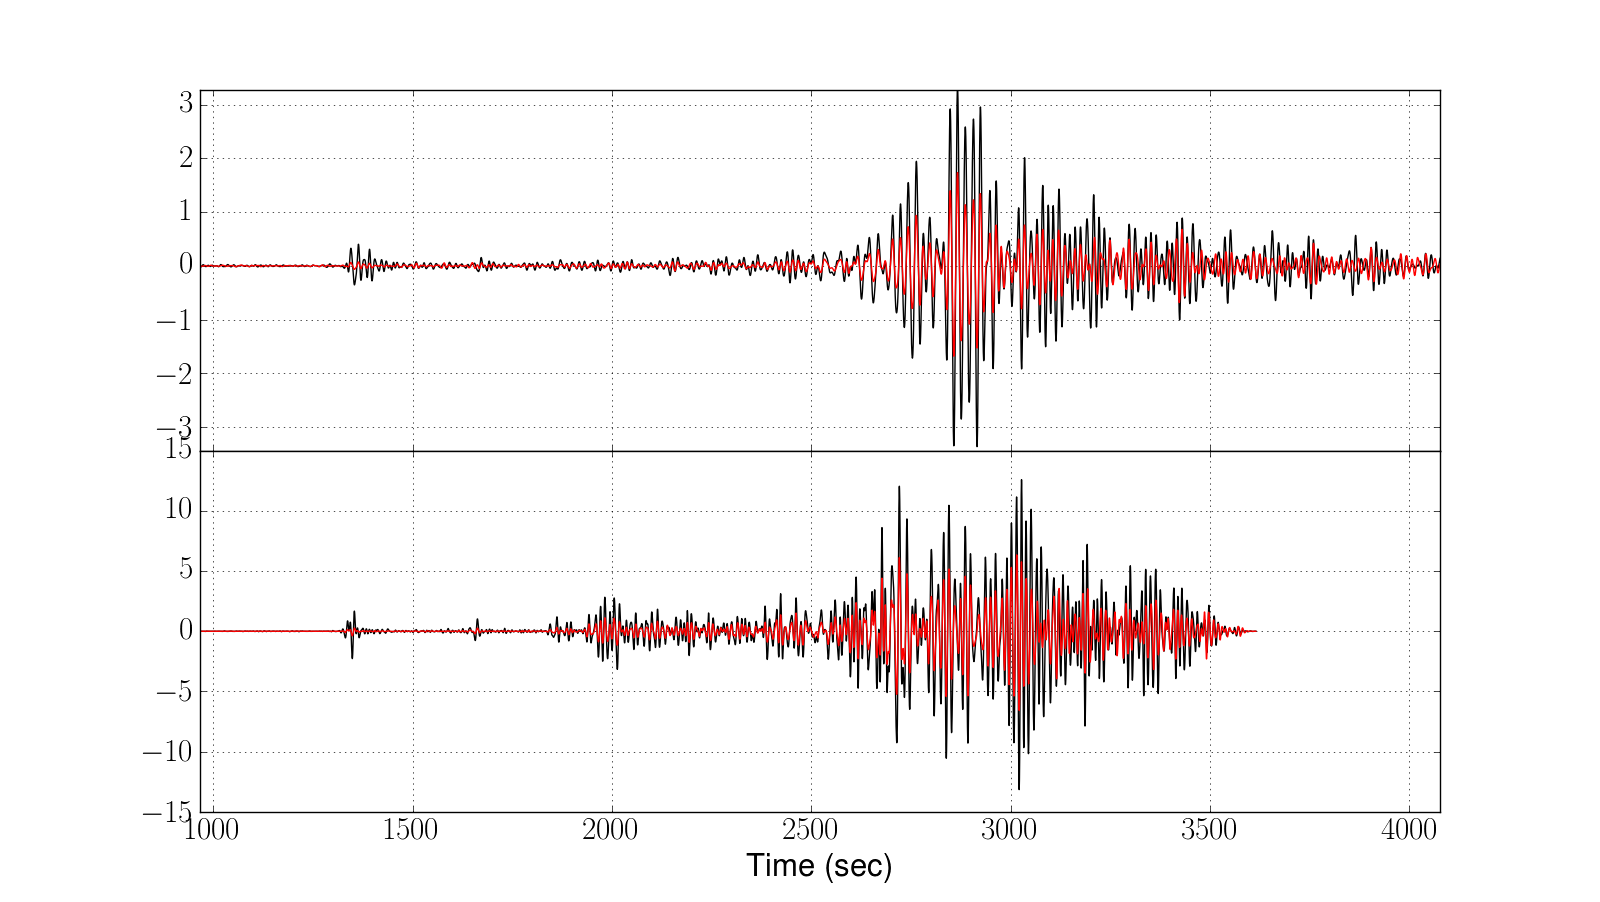
\includegraphics[width=0.5\textwidth]{rr_ta}}
\caption{Teleseismic event filtered at dominant period 20s. Note the phase matching of transverse acceleration and rotation rate, as well as the calculated value of horizontal phase velocity, c=3.81 km/s.}
\label{fig:rr_ta}
\end{figure}

\subsubsection{Peak correlation coefficient}
Correlations are a useful measure of similarity between two signals. It has been shown previously that for collocated measurements of vertical rotation rate and transverse acceleration, high values ($>0.9$) of zero lag correlations can be obtained in time windows centered around surface wave arrivals. %citation
Zero lag correlation coefficients are routinely computed for events measured by G [Salvermoser 2017], %citation
and are used in this study as a filtering tool to highlight "bad" events that exhibit low signal to noise ratios, or dissimilar waveforms which may arise due to non-physical effects (e.g. instrumental effects). Here, the largest correlation coefficient obtained for a seismogram is labeled the peak correlation coefficient (PCC), and is used as a representation of data quality for an event.


\subsection{Magnitude scales}
Here we discuss the common magnitude scale equation, and propose using a modified version of the equation as a method for comparing amplitude decay of various observables. Amplitude based magnitude scales provide empirically derived relationships between maximum trace amplitudes and source-receiver distances. Magnitude scales offer useful and quick estimates of relative sizes of earthquakes in a simple, standard  manner. 
The International Association of Planets Seismology and Earths Interior (IASPEI) Working Group on Magnitudes  proposed a modified version of the original surface wave magnitude equation proposed by Karnik et al. and Vanek et al., %citation
which is compatible for use with modern day broadband seismic instruments [Borrmann \& Bergman 2000].

In this work, we adhere strictly to these standard procedures provided by IASPEI as an outline for defining our own empirical magnitude scales. In turn, we use these derived scales as a tool for quantifying amplitude decay for different measured observables.

\subsubsection{Standard Procedures}\label{standproc}
The Working Group on Magnitudes' standard procedures gives the revised surface wave magnitude equation for broad-band instruments as,
\begin{equation}\label{eq:mag}
	M_S^{BB} = log_{10}(V/2\pi) + B\cdot log_{10}(\Delta) + C, 
\end{equation}
where the constants $B=1.66$ and $C=0.3$ control amplitude decay and order of magnitude, respectively. The parameter V should be the maximum trace amplitude (in nanometers second$^{-1}$) in the surface wave train, for a seismogram proportional to velocity, measured on the vertical component. 

Further criteria given by IASPEI posit that the period of the surface wave should lie within 3 s $\le$ T $\le$ 60 s, while epicentral distances should be between 2$^\circ \le \Delta \le 160^\circ$. It is further recommended that only shallow focus earthquakes should be considered, as medium to deep events are less capable of generating strong surface waves. %citation
Maximum trace amplitudes are described as one half the largest peak to adjacent trough deflection, and associated period are given as two times the temporal difference between peak and adjacent trough. All events and processing steps in this paper adhere to these guidelines.

\subsubsection{Instrumental proxies for Love and Rayleigh waves}\label{proxy}
A standard procedure for determining surface wave magnitude scales is to take amplitudes measured on the vertical component of translation. This is because vertical translation should only be sensitive to the vertical motions of Rayleigh waves, whereas vector sums of horizontal components can be influenced by both Love and Rayleigh waves. In the same vein, velocity measured on the transverse component should only show sensitivity to Love waves (and radial components should only be sensitive to the horizontal component of Rayleigh waves). This is, however not common practice,  due to the necessity of rotating horizontal components to the correct azimuth, which can be affected by ray paths and local site effects. The G-ring, which is: 1) insensitive to translations and 2) proportional in phase and amplitude to transverse acceleration, should however only be sensitive to Love waves in the surface wave train, irrespective of azimuth.  

In this study we use our instruments as physical wave-filters, in order to separate phases in the surface wave train. This allows us to study the influences of Love waves and Rayleigh waves individually. By comparing the vertical and transverse components of translations, to the vertical component of rotation, we can understand, by proxy, the wave types they are sensitive to.

\subsubsection{Application of rotations to magnitude scales}
The surface wave magnitude equation is defined for peak vertical velocity amplitudes in the surface wave train. In order to give a fair comparison using derived magnitude scales, a complementary rotation parameter is necessary. In Section \ref{phasevel}, an equation is given that relates rotation rates $\Omega$ with accelerations $\ddot{u}$. It would make the most sense, then, to compare velocities $\dot{u}$ with rotations $\omega$ (by integrating both sides). However, without previous work to draw precedence from, and for completeness, we present observations of both rotations and rotation rates in this study.

\section{Event choice}
The G-ring has been continuously recording at its current resolution since May, 2009 [Citation for mirror upgrade?]. 
The time range for events used in this study spans June 1, 2009 to September 1, 2016. An initial earthquake catalog was fetched from the Harvard Global Centroid Moment Tensor (GCMT) [Ekstr\"om et al. 2012 ?], %citation 
with events filtered by acceptable magnitude, source depth and epicentral distance from Wettzell, Germany. At this point we imposed the restriction that the derived 'magnitude' as given by our magnitude equations, should fall as close to the given surface wave magnitude as possible. This ensures that our derived scales do not stray too far from established scales. This meant that only events with centroid moment magnitude values of $6 \le M_{\text{wc}} < 8$ (as published in the GCMT catalog), were considered;   surface wave magnitude and moment magnitude are approximately equal in this range [Shearer 2009]. %citat
Zero-lag cross correlations of transverse acceleration and rotation rate were taken in order to calculate peak correlation coefficients (Section \ref{sec:dataproc}). Events were not considered if their peak correlation coefficient did not meet the criterion PCC $< 0.7$. 

These choices for event criteria narrowed the catalog down to roughyl 500 events in the given time period. Each event was appropriately filtered and processed (Section \ref{sec:dataproc}), and waveforms were individually inspected. Waveforms that exhibited anomalous behavior (i.e. unexpected high amplitude peaks outside the surface wave train, high signal-to-noise ratio etc.) were rejected. A final event catalog of 243 events was reached, shown on a world map in Figure \ref{fig:event_map}.

\begin{figure*}
\centerline{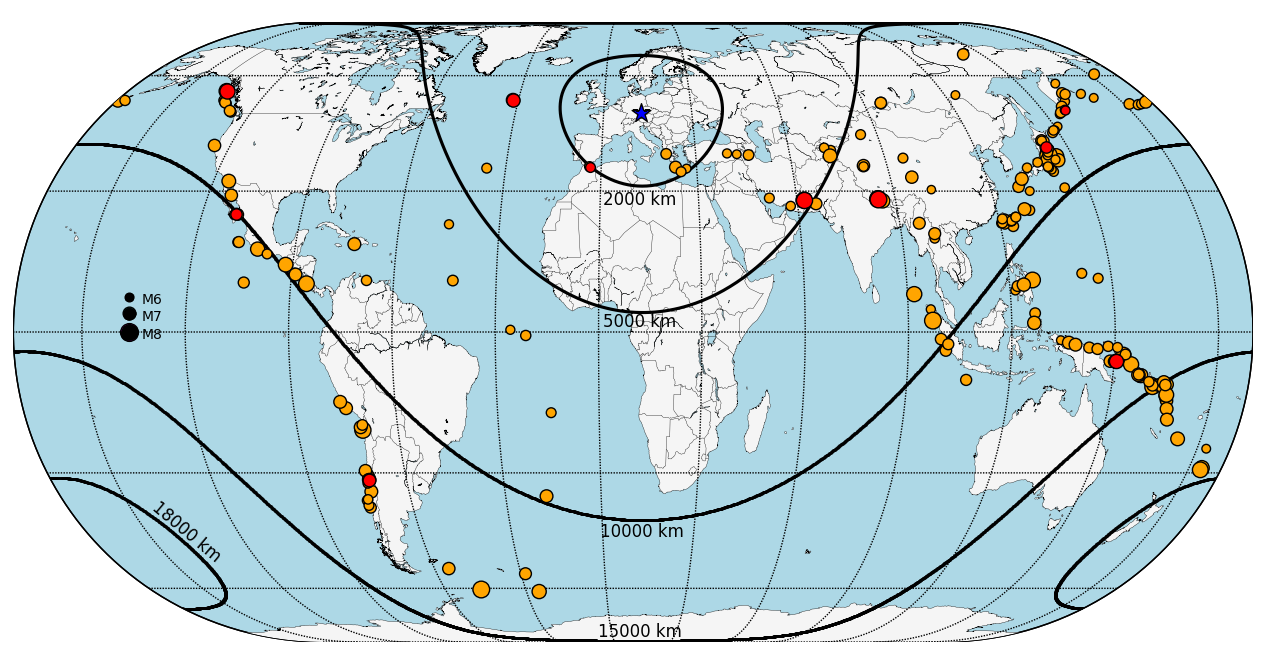
\includegraphics[width=.8\textwidth]{event_map}}
\caption{Event map. Size represents moment magnitude (M$_{wc}$). Orange dots show observed earthquakes used in magnitude scale derivation. Red dots show the ten events chosen for generation of synthetic seismograms. Black lines are equidistant points from the blue star, which represents the location of G in Wettzell, Germany (49.144$^\circ$N,12.87$^\circ$E).}
\label{fig:event_map}
\end{figure*}

\section{Methods}
\subsection{Data Processing}\label{sec:dataproc}
Events were processed in a similar fashion as the processing outlined in Salvermoser 2017. %cite johannes
Raw, continuous translation data in North, East and vertical components, as well as vertical rotation rate data, was fetched based on event origin time. Instrument response correction produced translation seismograms proportional to units of velocity (nm s$^{-1}$). Epicentral distances ($\Delta$) and theoretical backazimuth values were calculated from station-receiver latitude longitude pairs, and events were separated into categories of close ($\Delta < 3^\circ$), local ($\Delta <100^\circ$) and far ($\Delta \ge 100^\circ$). Horizontal components were rotated into the transverse, radial, vertical coordinate system by the appropriate theoretical backazimuth. Measurements from ring laser gyroscope instruments do not require frequency dependent instrument correction [Sagnac ????], %citation
therefore only a simple scale factor was necessary to retrieve seismograms proportional to rotation rate (nrad s$^{-1}$). Rotation rate traces were integrated to provide measurements of rotation (nrad), and transverse velocity was integrated to retrieve transverse acceleration, which was subsequently used to calculate correlations with vertical rotation rates.
A bandpass filter was applied to all traces for periods between 3 s $\le$ T $\le$ 60 s, in accordance to the IASPEI standard procedures. Peak amplitudes were chosen by finding minimum and maximum trace values and the largest associated peak or trough, respectively. The larger of the two was chosen, alongside the associated arrival time and dominant period, taken as two times the distance between peak and adjacent trough. 
Theoretical considerations used to restrict search to the surface wave train proved inconsistent over a large number of events, so maximum amplitudes in the entire trace were considered. Through manual inspection, picked amplitudes that fell outside the surface wave train (which occurred very infrequently) were rejected. An example of the waveforms and amplitude picking is shown in Figure \ref{fig:obswave}.


\begin{figure}
\centerline{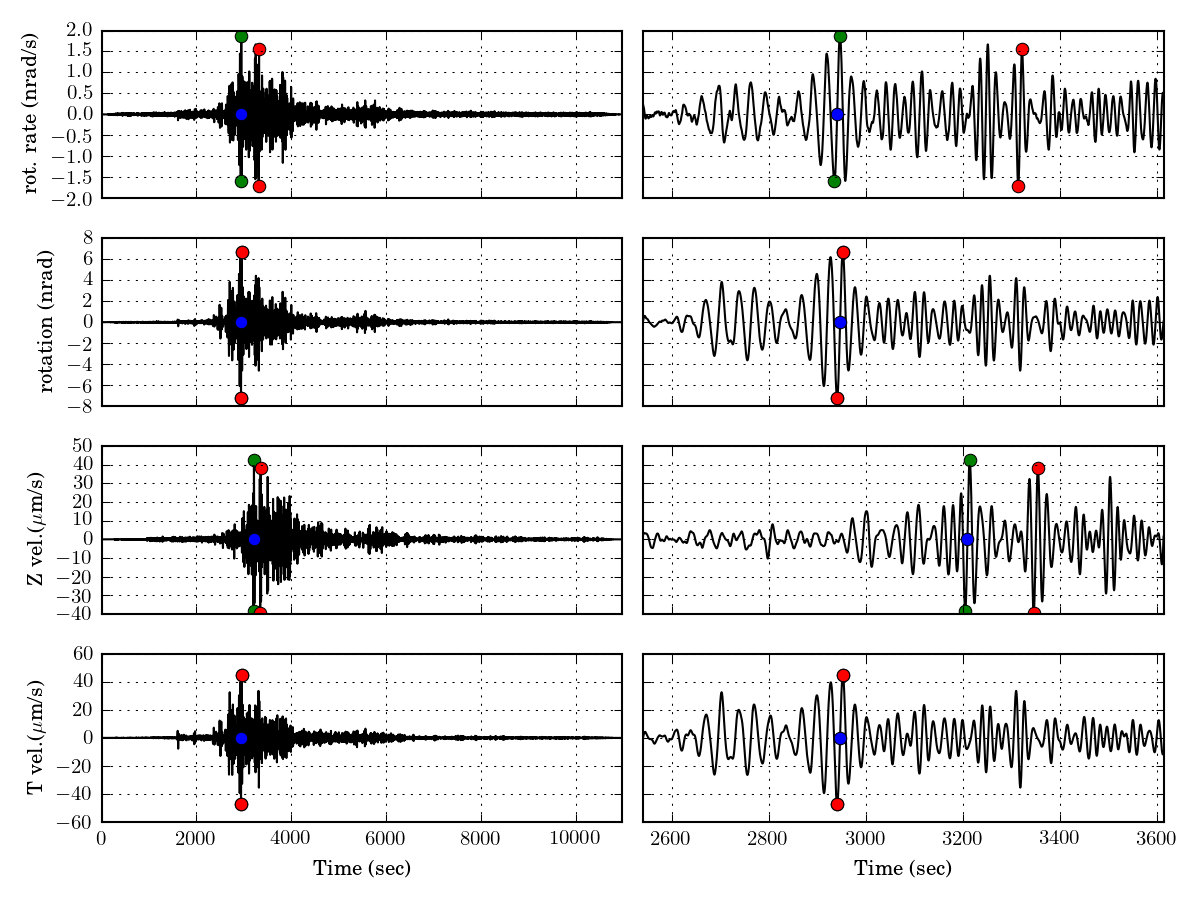
\includegraphics[width=0.5\textwidth]{amp_picking}}
\caption{Left: Seismograms for observed rotation rate, rotation (measured by G), and two components of translation (colocated STS-2), vertical and transverse components.\newline Right: Zoomed in section of seismograms, showing peak to peak amplitude choice (blue dot). Red and green dots show largest peak to adjacent trough distance and largest trough to adjacent peak distance, respectively. Note the visible difference in arrival times of the Love wave (as seen on rotation and transverse components), and the later arriving Rayleigh wave (as seen on the vertical component). }
\label{fig:obswav}
\end{figure}


\subsubsection{Zero-lag correlations}
To calculate peak correlations, traces of transverse acceleration and vertical rotation rate were segmented into small time windows based on the event-station distance. In each time window, a zero-lag correlation was performed, and a single value of correlation produced. From the entire trace, the max value was taken to represent the peak correlation coefficient. For most waveforms, the peak correlation coefficient lie in the surface wave train. As mentioned previously, these peak correlation values are used extensively as a ranking system for events, providing a quickly attainable measure of waveform quality.

\subsection{Curve fitting}
To quantify amplitude decay, magnitude scale coefficients were fit to the data using a simple linear regression. Equation \ref{eq:mag} represents a relationship between magnitude and amplitude for a single event. Using Equation \ref{eq:mag}, a collection of $n$ events can be represented in the form, 
\begin{equation}
	\begin{pmatrix}
		log_{10}(\Delta_{1}) & 1 \\
		log_{10}(\Delta_{2}) & 1 \\
		\vdots  & \vdots \\
		log_{10}(\Delta_{n}) & 1 
	\end{pmatrix}
	\begin{pmatrix}
		{B}\\
		{C}
	\end{pmatrix}
	=
	\begin{pmatrix}
		M_{\text{wc}_1} - log_{10}({V_1}/{2\pi})_{\text{max}} \\
		M_{\text{wc}_2} - log_{10}({V_2}/{2\pi})_{\text{max}} \\
		\vdots  \\
		M_{\text{wc}_n} - log_{10}({V_n}/{2\pi})_{\text{max}}
	\end{pmatrix},
	\label{eq:linearreg}
\end{equation}

\noindent which can be further condensed to the form, $\mathbf{Gm = d}$. The unknowns B and C are represented in the vector {\bfseries m}, and can be solved for through the normal equation $\mathbf{m} = \mathbf{(G}^{T}\mathbf{G})^{-1}\mathbf{G}^T\mathbf{d}$.
By determining values of B and C, we create an empirical magnitude scale that best describes the amplitude decay behavior of our events. In Equation \ref{eq:linearreg}, we impose that our derived magnitude value should be as close to an events given moment magnitude as possible, by setting $M_S^{BB}$ equal to the value of $M_\text{wc}$ retrieved from our event catalog. 

95\% confidence intervals were constructed for each parameter of the vector $\mathbf{m}$. These were calculated with the variance of estimates of the $j$th parameter of $\mathbf{m}$ by the equation $\hat{m}_j \pm c \sqrt{\hat{var}(\hat{m}_j)}$, where the value of c is given as 1.96 for a confidence interval of $\alpha = 0.95$.

\section{Synthetic seismograms}
Due to the unique instrumental setup of the G-ring, there are currently no other rotational instruments with as much temporal coverage to draw comparisons from. It should be mentioned that there are other available rotation instruments which allow for single event case study analyses [Donner 2017 PFO?] [iXblue?] [PFORLAS], however large catalogs like that available from the G-ring are currently unavailable. One possibility for gathering more observations would be through array derived rotations as a substitute for direct rotation measurements [Spudich ?]; this option was noted during analysis, however it proved difficult finding sufficient long-term arrays with the optimal station spacing. In the future if this type of data became available, it would provide a very useful addition of information to this study. In lieu of observations, we instead turn to waveform modeling to generate synthetic seismograms, with which we recreate our experimental setup and provide a comparable set of synthetic observations.

The seismic wave propagation code Specfem3D Globe was employed [cite specfem]. A realistic global model featuring 3D crust and mantle models was used, and the simulation featured effects that might have potential influence on surface waves at the periods of interest. These effects include: ocean loading, Earth's ellipticity, topography, self gravitation, Earth's rotation and 1-D attenuation. Event locations and moment tensors were taken from 10 real seismic events present in the observation catalogs. Events were chosen based on observation data quality, as well as event location and depth, so as to provide a varied distribution of source-receiver pairings. Table \ref{tab:syn_events} provides detailed information on the chosen events. 

In each simulation, events were initiated as point sources. The simulation corner frequency was set to 10 seconds, and simulations were run for one hour simulation time. As computational cost is independent of number of stations, more than one hundred stations were included; Global Seismic Network (GSN) locations were used, as well as location of the G-ring, and the German observatory station F\"urstenfeldbruck. The number of simulated stations was X, and the number of station-receiver pairs X (with some station-receiver pairs falling outside the distance bounds specified in Section \ref{standproc}).

\begin{table*}
\begin{minipage}{150mm}
	\begin{center}
		\begin{tabular}{ |c|c|c|c|c|c|c|c| } 
		\bf{Date} & \bf{Time (UTC)} & \bf{Lat($^\circ$)} & \bf{Lon($^\circ)$} & \bf{Depth(km)} & \bf{M$_{\text{wc}}$} &\bf{Flinn-Engdahl Region} &\bf{Peak Corr. Coeff.}\\ \hline
	2010-07-18 & 13:34:59 & -5.93 & 150.59 & 35.0 & 7.32 & New Britain Region, P.N.G. & 0.98\\
	2011-09-16 & 19:26:41 & 40.27 & 142.78 & 35.0 & 6.67 & Off East Coast Of Honshu, Japan & 0.99\\
	2013-01-05 & 08:58:19 & 55.39 & -134.65 & 10.0 & 7.53 & Southeastern Alaska & 0.95\\
	2013-04-16 & 10:44:20 & 28.03 & 62.0 & 80.0 & 7.74 & Southern Iran & 0.98\\
	2013-04-19 & 19:58:40 & 49.97 & 157.65 & 15.0 & 6.06 & East Of Kuril Islands & 0.99\\
	2015-02-13 & 18:59:12 & 52.65 & -31.9 & 16.7 & 7.07 & Reykjanes Ridge & 0.99\\
	2015-04-25 & 06:11:26 & 28.15 & 84.71 & 15.0 & 7.88 & Nepal & 0.99\\
	2015-09-13 & 08:14:12 & 25.14 & -109.43 & 10.0 & 6.6 & Gulf Of California & 0.98\\
	2015-09-16 & 23:18:41 & -31.56 & -71.43 & 28.4 & 7.1 & Near Coast Of Central Chile & 0.99\\
	2016-01-25 & 04:22:02 & 35.65 & -3.68 & 12.0 & 6.38 & Strait Of Gibraltar & 0.99\\
		\end{tabular}
    		\caption{List of events used as synthetic sources in Specfem3D. Peak correlations are used as a measure of waveform quality, and only events with the highest values were used, in order to provide the best comparisons of synthetics with observations. Events were also chosen based on a diverse coverage of magnitudes and epicentral distances from the ring laser stationed in Wettzell, Germany. Event information taken from the GCMT catalog.}
		\label{tab:syn_events}
	\end{center}
	\end{minipage}
\end{table*}

The direct outputs of Specfem3D were adjusted to produce displacement (in units of meters) in the transverse, radial and vertical components, by rotation with respect to the theoretical backazimuth. Direct rotation (in units of radians) in the same coordinate system was also outputted. During processing, translation seismograms were differentiated to retrieve velocity waveforms, and rotation was differentiated to produce rotation rate waveforms. A work flow identical to that used for observations was employed to calculate peak trace amplitudes, and a magnitude equation was fit to the data for comparison.

\section{Results}\label{sec:results}
\subsection{Derived magnitude scales}
Decay characteristics of rotations and translations were derived by solving for constants B and C in Equation \ref{eq:linearreg}. The values for each scale are presented in Table \ref{tab:scales}. For an additional check on site-dependent data quality, the same analysis was performed on translation observations taken at the geophysical observatory F\"urstenfeldbruck, Germany (FUR; 48.163$^\circ$N, 11.275$^\circ$E), located roughly 200 km south-west of Wettzell. Though a smaller subset of events was used due to data availability, the results confirmed those given at Wettzell. 


\begin{figure*}
\centerline{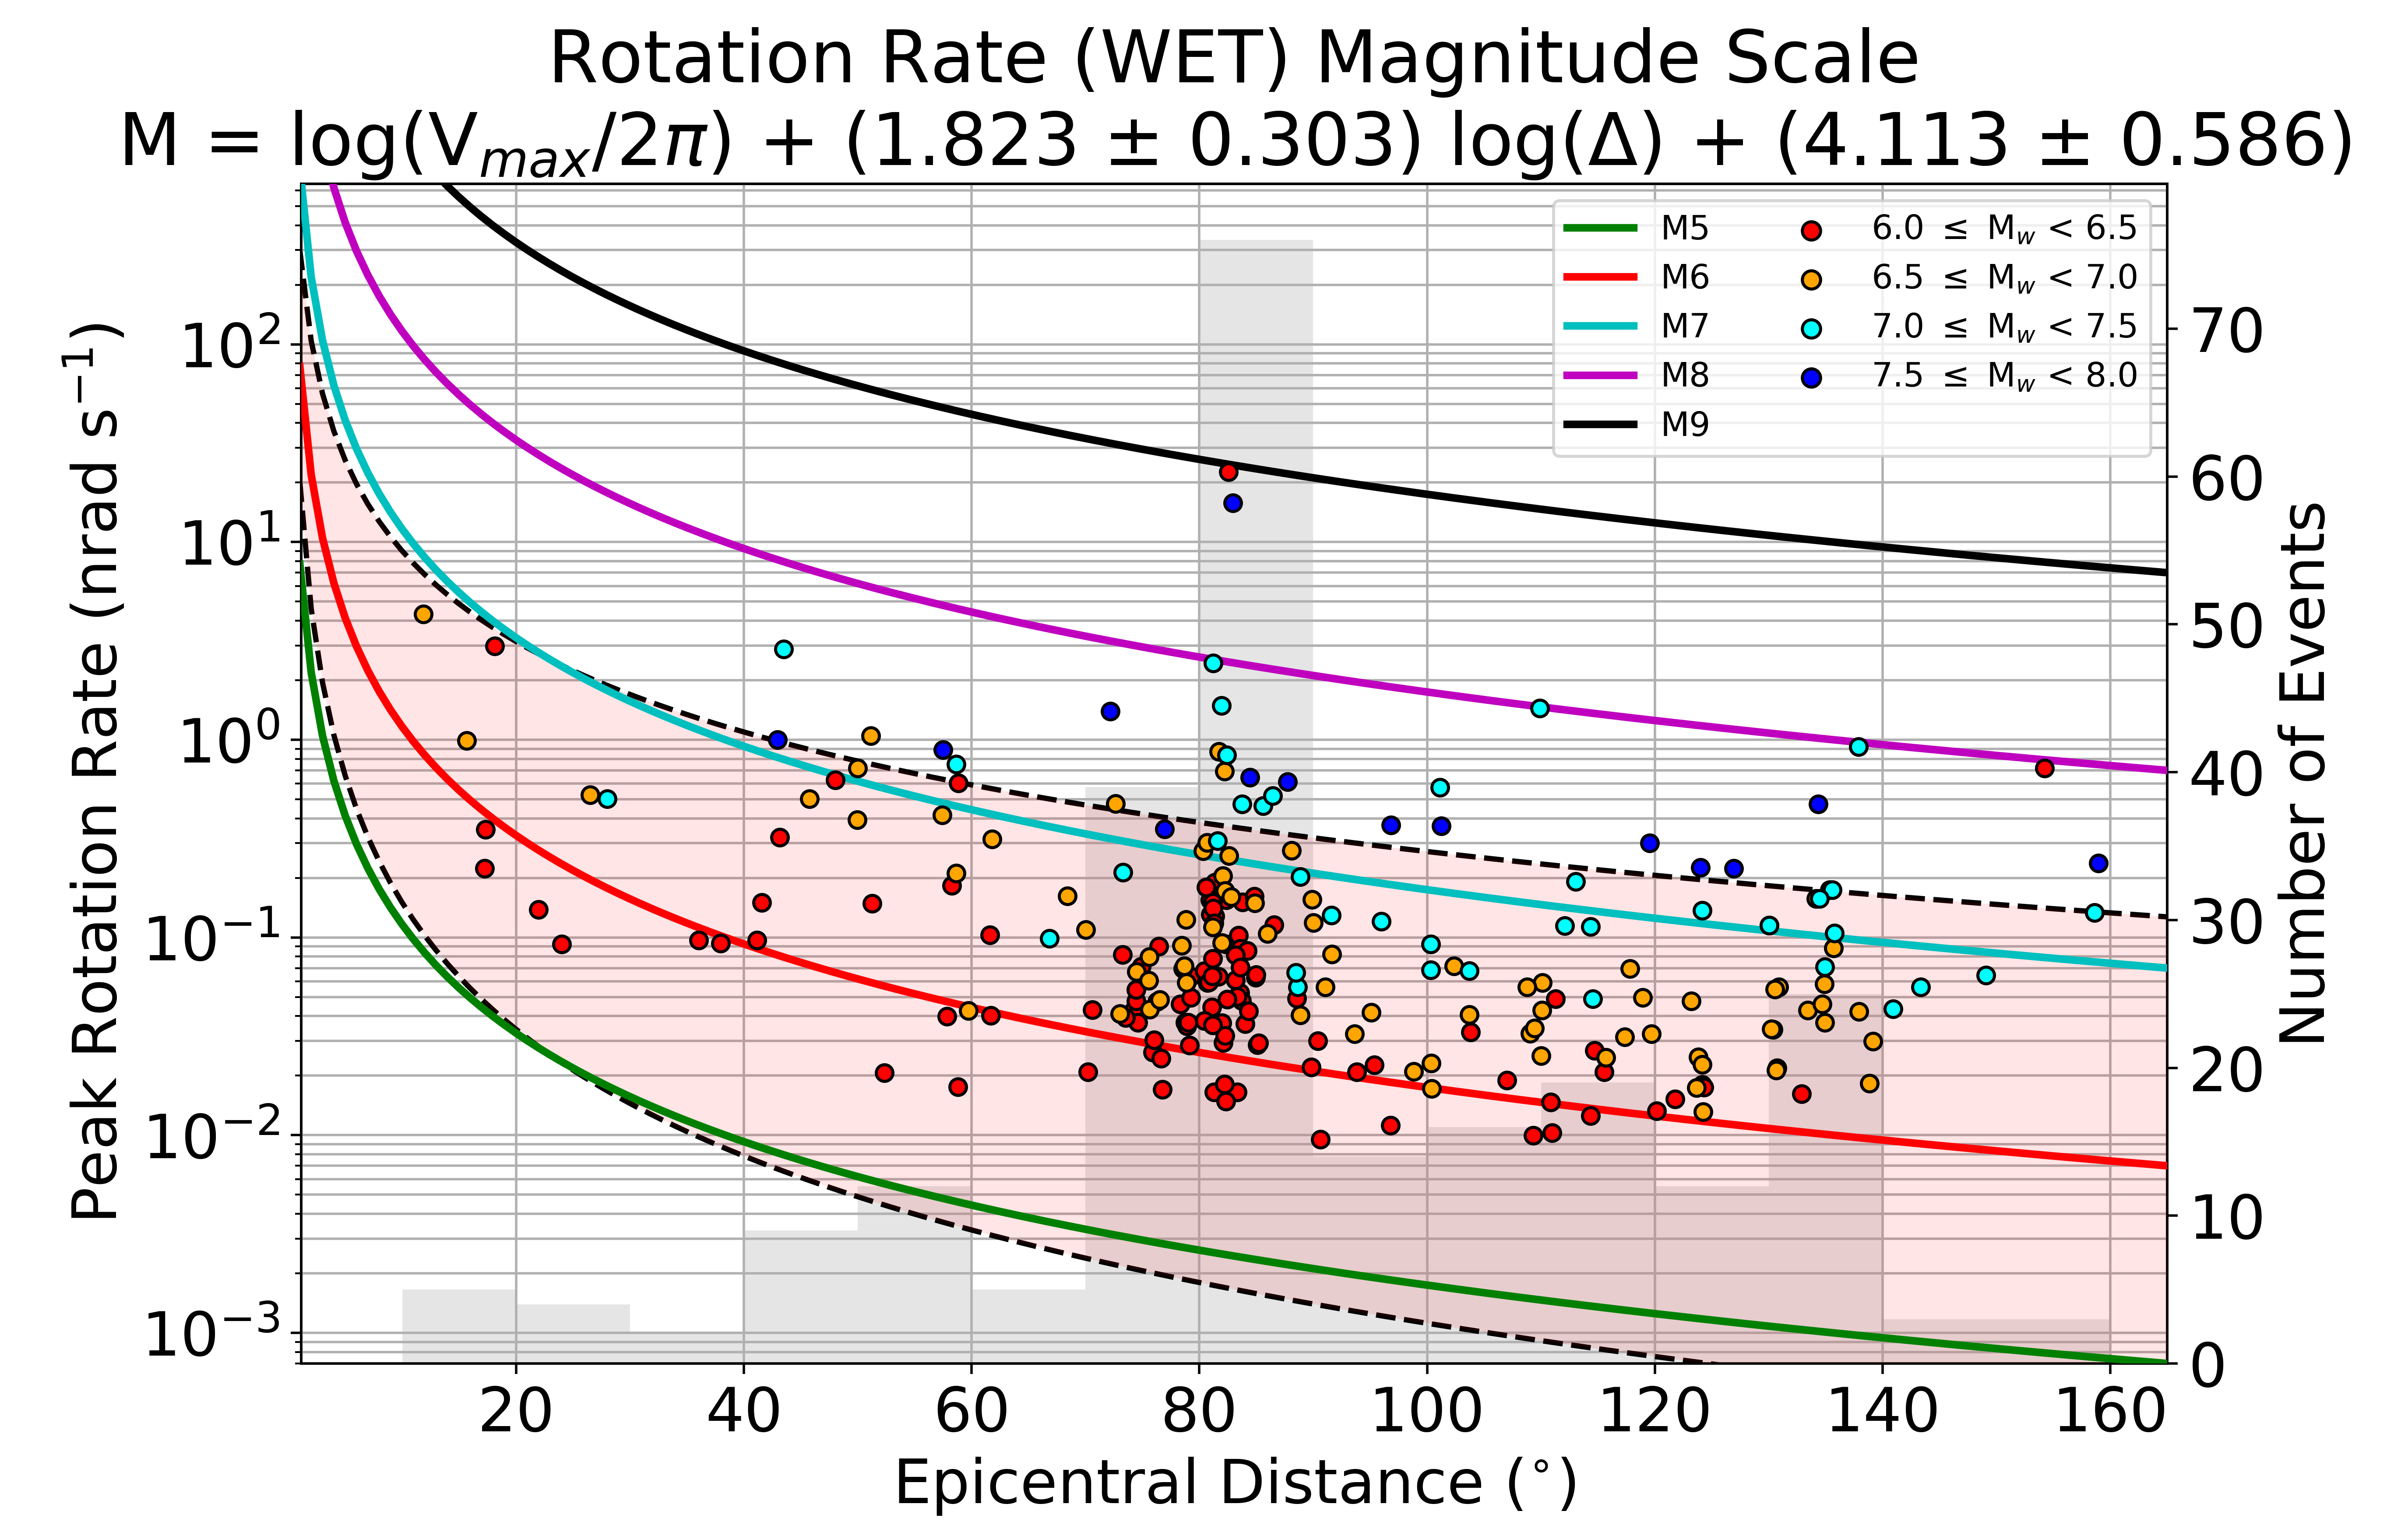
\includegraphics[width=.8\textwidth]{RR_WET}}
\caption{Rotation rate magnitude scale for observations. Event magnitudes separated by bins of 0.5 and denoted by color. Magnitude equation plotted by integer values as solid color lines. 95\% confidence interval for M6 shown by the shaded red area, bordered by black dashed lines. The number of events for each epicentral distance bin shown by gray bars in the background.}
\label{fig:rr_obs}
\end{figure*}

%translation scales
The value of B covers a large range, from 1.084 to 1.823 for vertical velocity M$^{WET}_{Z}$ and rotation rate M$^{RLAS}_{RR}$, respectively. Rotation M$^{RLAS}_{RT}$ falls closest to the standard IASPEI value of B=1.66. Velocity values match quite consistently between Wettzell and F\"urstenfeldbruck, with FFB showing slightly higher amplitudes, as seen in the value of C, which controls the order of magnitude of expected amplitudes. In comparing these two stations, consideration should be given to the subsurface composition; the geodetic observatory in Wettzell overlies granitic bedrock, while F\"urstenfeldbruck sits atop a sedimentary basin, which are known to amplify passing seismic waves. It is therefore not surprising, and perhaps expected, that we observe on-average larger amplitudes at F\"urstenfeldbruck. This is visible in the transverse component, sensitive to Love waves, in Figure \ref{fig:velocity_comp}, however the vertical component, sensitive to the vertical component of Rayleigh waves, does not reflect this. 

Variations of velocity based scales from the surface wave magnitude equation are large, but not as unsurprising as they first appear. It has been proposed that the modern surface wave magnitude equation has a systematic distance bias, which tends to under predict amplitudes at greater distances [Herak Herak 1993]. Previous works have proposed corrected values of the coefficients B and C, using a global catalog [Herak Herak 1993] and a European regional dataset [Ambraseys Free 1997]. These corrections match well with the vertical velocity scales derived in this work; the values (adjusted for the change of units in the IASPEI scale) are presented in Table \ref{tab:scales} as $M_S^{HH}$ and $M_S^{AF}$ for scales proposed in Herak Herak [1993] and Ambraseys-Free [1997], respectively. 

There exists a noticeable difference between values of B for transverse and vertical velocities. The vertical velocity scale is expected to present an identical setup to the broadband surface wave magnitude equation, however it gives with the largest discrepancy, for both stations WET and FUR.  Transverse velocity, which should sample Love waves, same as rotations (see \ref{proxy}), shows a larger value for B as compared to vertical velocity.

\begin{figure}
\centerline{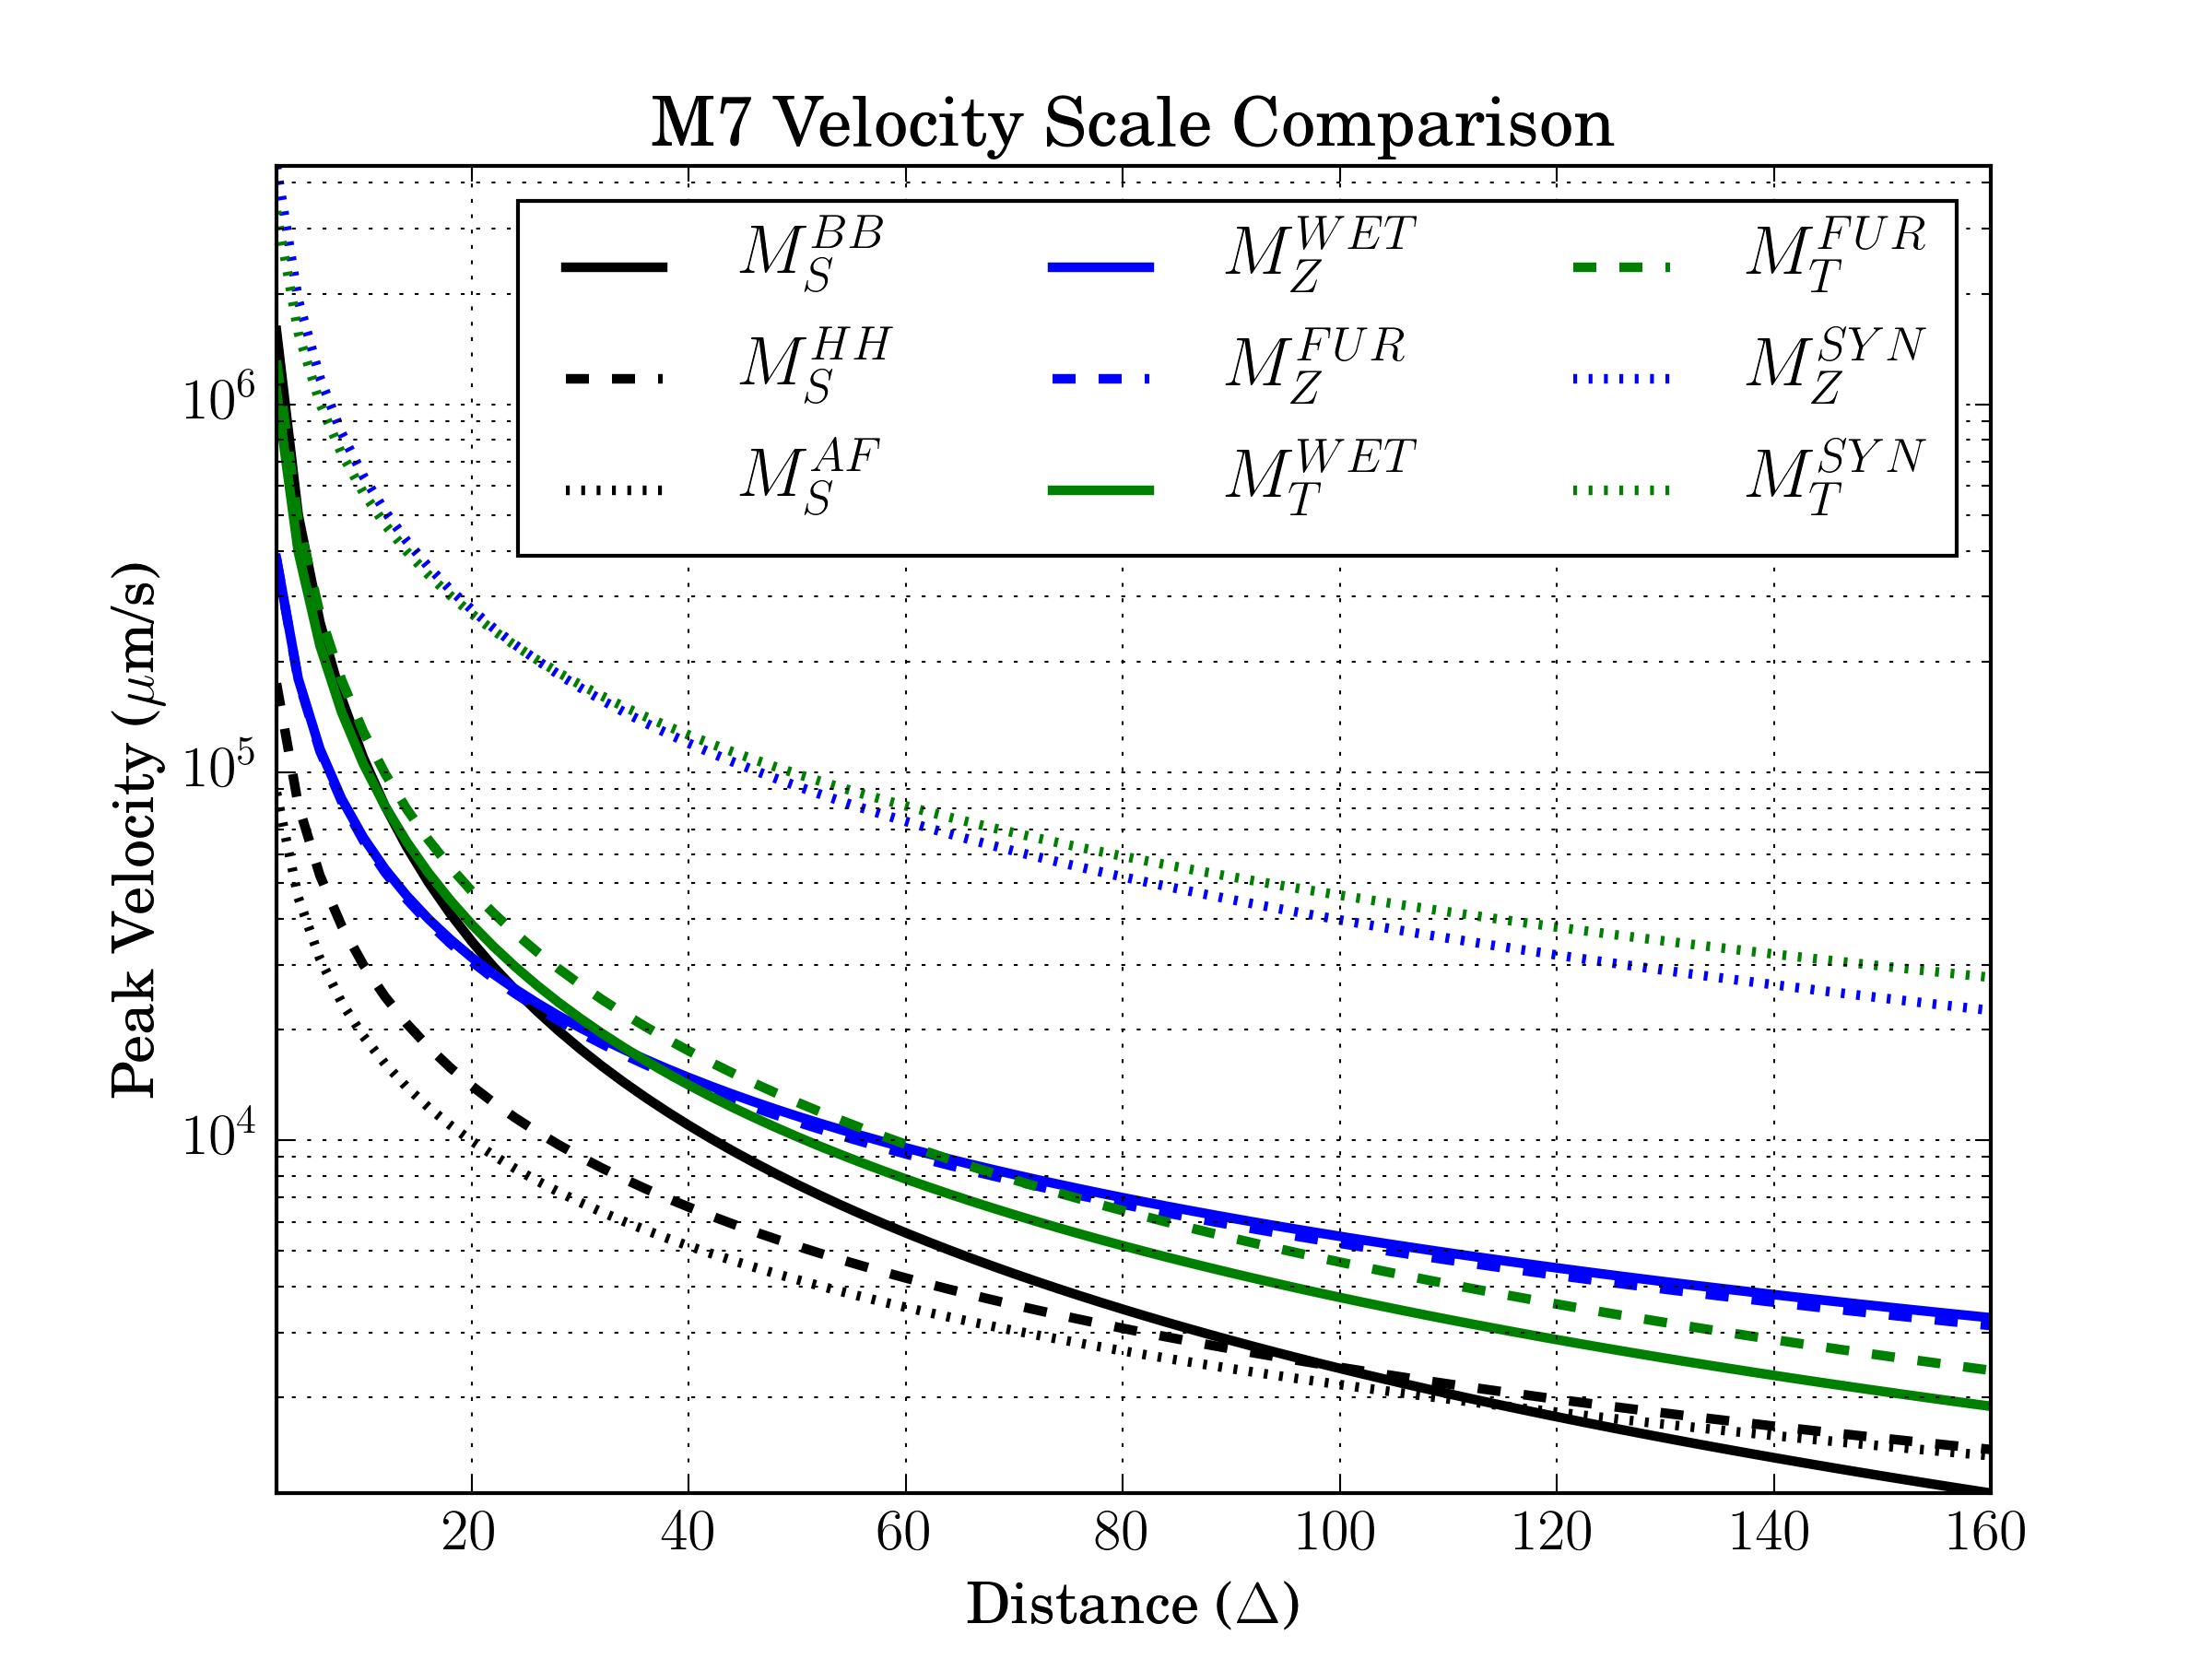
\includegraphics[width=.5\textwidth]{velocityscales}}
\caption{A comparison of velocity based scales for stations WET, FUR and synthetic scales, with the IASPEI scale used as reference. Peak amplitudes given in units of nanometers/s}
\label{fig:vel_scale}
\end{figure}

\begin{figure}
\centerline{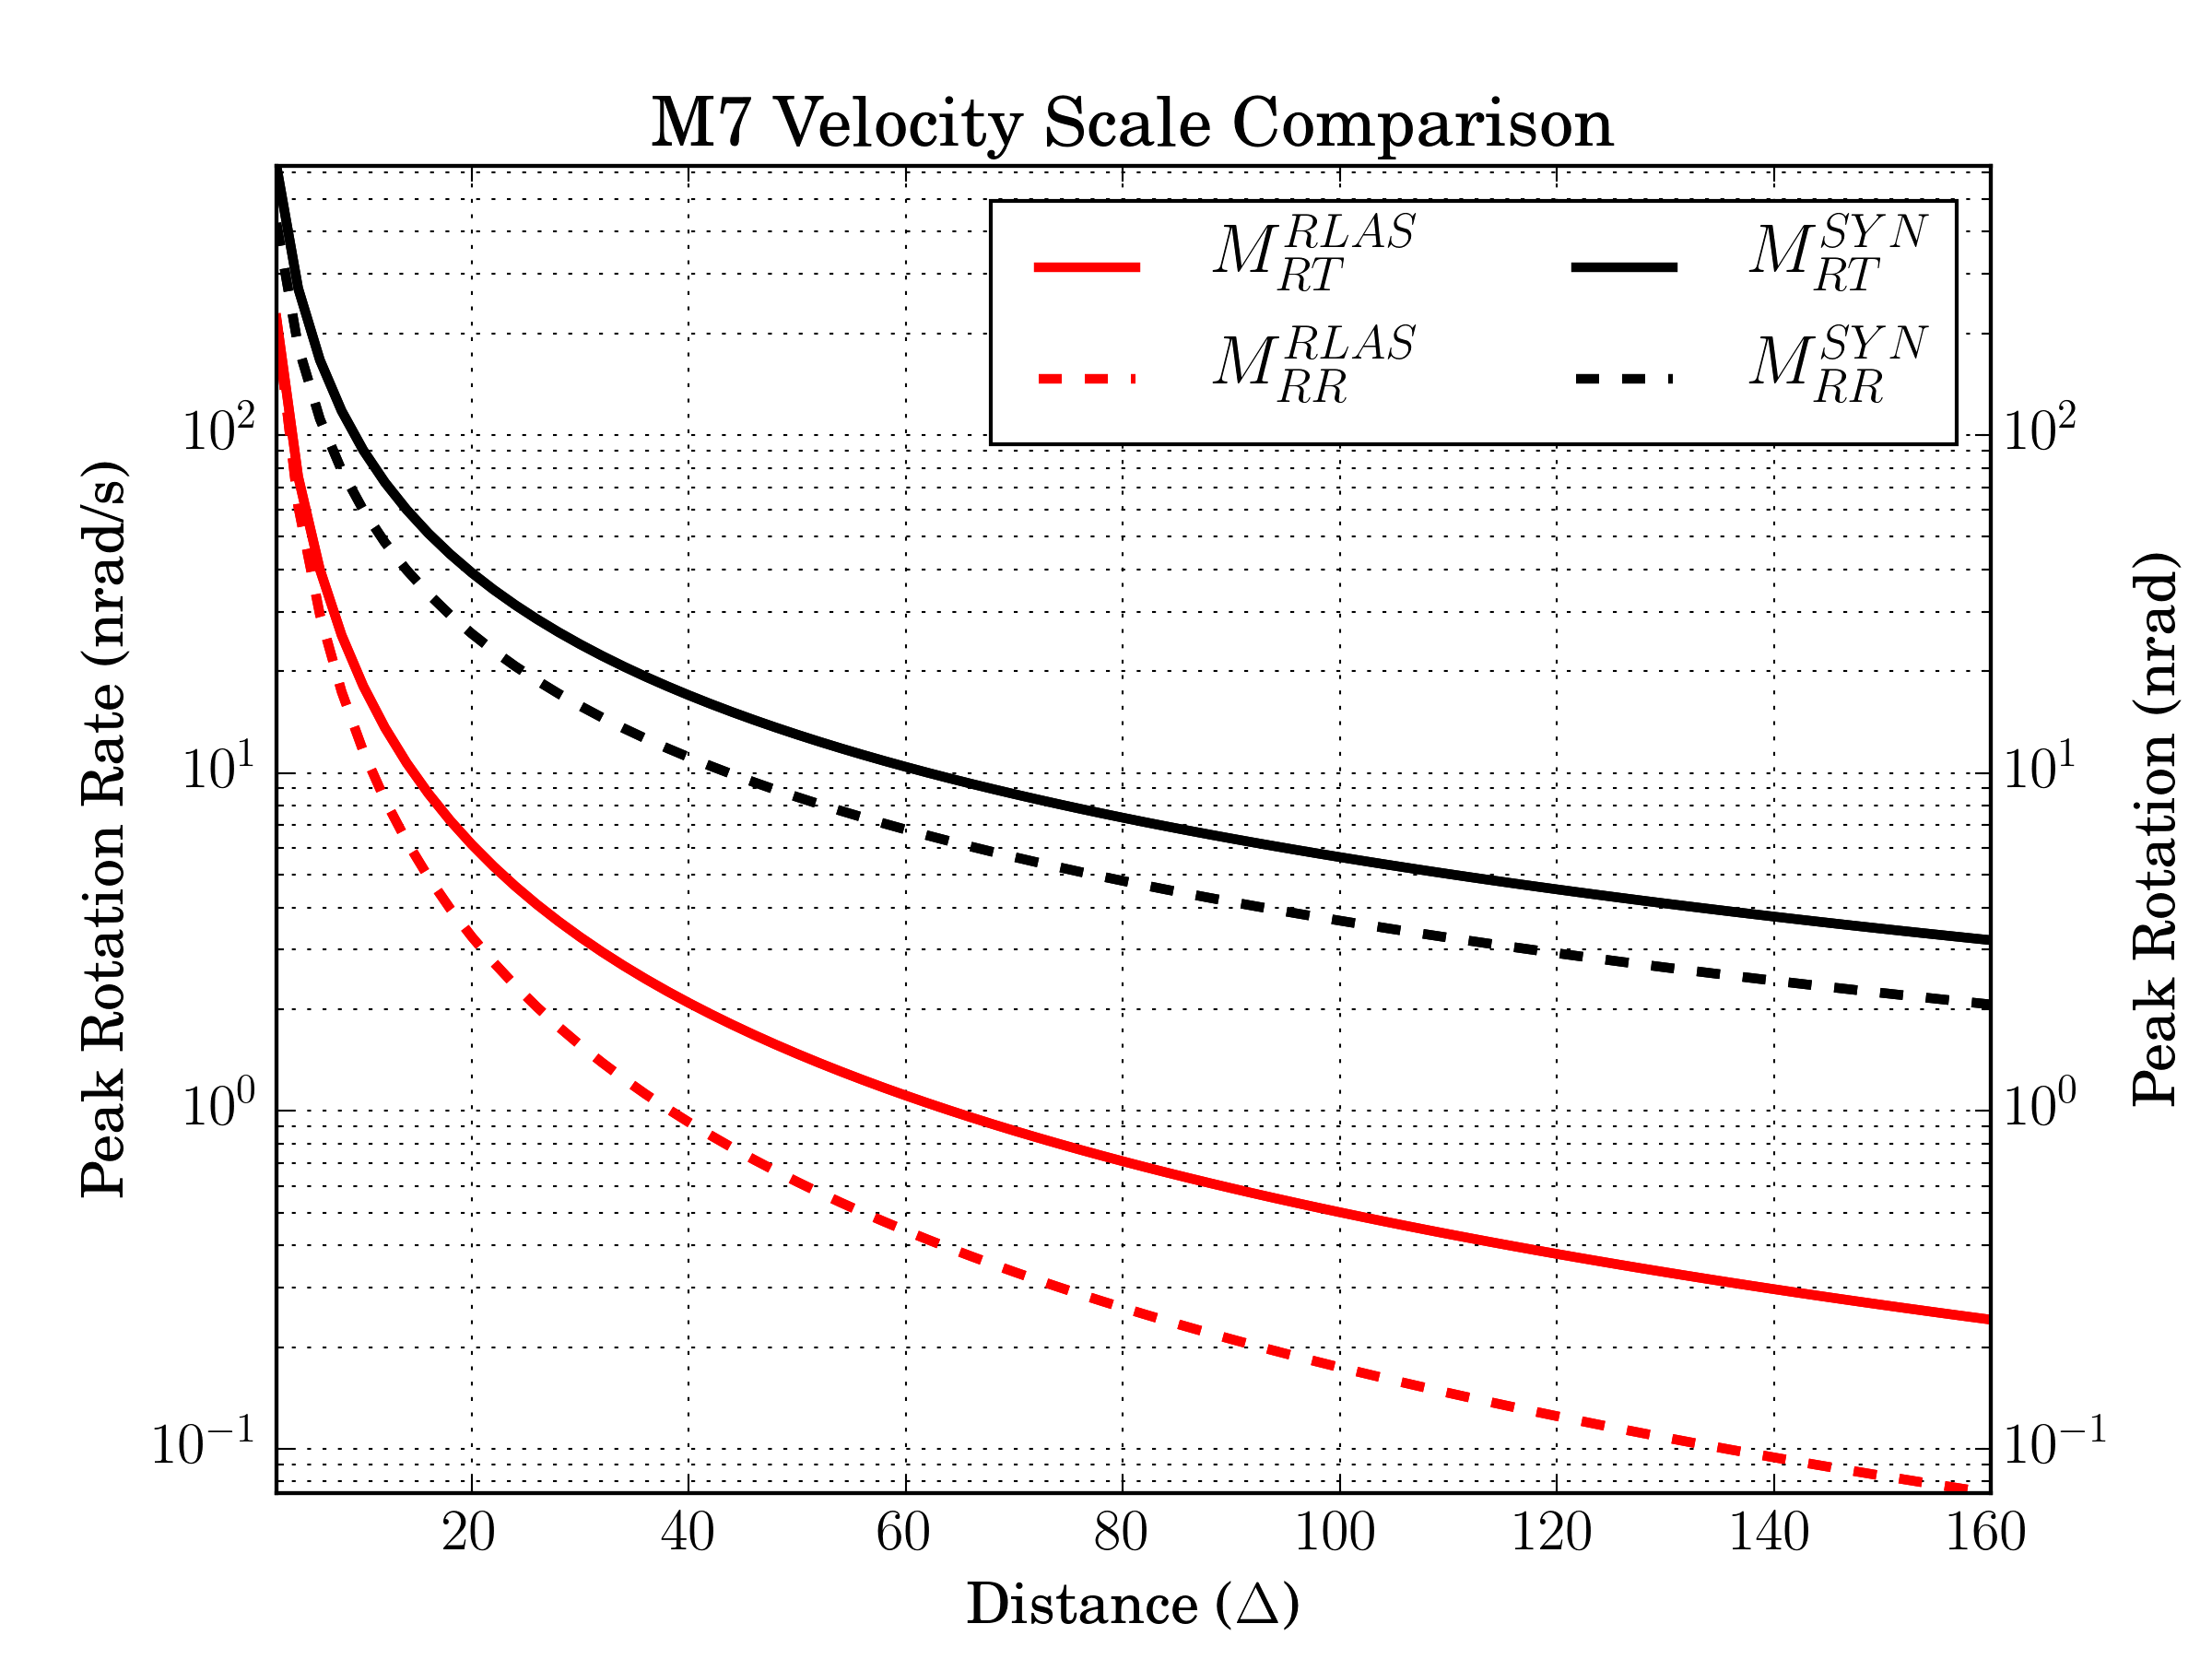
\includegraphics[width=.5\textwidth]{rrscales}}
\caption{A comparison of rotation based scales for station WET and synthetic scales. Peak amplitudes given in units of nanoradians/s}
\label{fig:rr_scale}
\end{figure}

It is to be expected that rotation rate shows a larger value for B as compared to rotation, as rotation is being compared with its time derivative, which contains amplified high frequency components and should exhibit faster decay with distance as the wave path filters out this high frequency energy. 

Confidence intervals, which can be viewed as a quantification of misfit between the fitted magnitude equation and the observations, shows the uncertainty of the observations due to the limitation of spatial coverage; in Figure \ref{fig:rr_obs}, the red shaded area shows the confidence interval of the M6 decay line. % add some explanation on confidence intervals
It should be noted that the magnitude scale is heavily controlled by its end members. Due to a lack of events at very close epicentral distances, it is difficult to constrain the decay here, and the few events at distances less than 20$^\circ$ have a strong influence on the derived value of B. It can also be seen that more than one third of the events used in this study fall around 80$^\circ$ epicentral distance, due to geographic constraints; many of these events occur around Japan. 

%Discussion: comparing regional view vs an averaging
\subsection{Observed and synthetic waveforms}
For each of the simulated events, synthetic seismograms were generated for all stations mentioned previously. Waveforms for station WET were compared for all possible components of translation and rotation. In one event (2010-07-18), a fore shock in the observations went unnoticed during event choice, which prevented useful comparison. In most other cases, P-wave and S-wave arrivals matched well. Later arrivals are not in agreement with very different behavior exhibited by arriving surface waves. This can be potentially explained by the use of point sources for such large magnitude earthquakes; the effects of the source time function as well as the rupture plane are not captured in our synthetics, and we therefore do not expect to match phases of surface wave arrivals. Consideration should also be given to the topographic and crustal models included, which affect the resulting surface wave waveforms. Fortunately we focus on peak amplitude measurements in this work, and therefore are not deterred by the misfit of waveforms. The broad frequency range (10-60s) also present difficulties in matching waveforms. Narrow pass filters (i.e. 20 second dominant period) capture similarities better, however in this study we aim to stick to the definition of the IASPEI surface wave magnitude equation, which calls for a broad frequency range.

%traces only extend one hour?

As to be expected, the observed waveforms present a much more complicated picture of arrivals. In most of the observations, noise levels are high enough that determining body wave arrivals is difficult compared to the synthetic models. Even for narrow pass filters, as in Figure \ref{fig:both}, observation and synthetic seismograms do not exhibit high correlations. Neverthless, peak amplitude picking in all 10 events falls in the surface wave train which allows for determination of magnitude scales - this allows us to make comparisons without relying on detailed waveform information.

Comparisons of transverse acceleration and rotation rate provide solid phase matching throughout the waveform, with the strongest correlation during the surface wave train, even for relatively wide bandpass filters (i.e. 10 to 60 seconds). This is true for both observations and synthetics, and also allows for the calculation of phase velocities. Because this is not the goal of this paper, we do not delve too far into the analysis of phase velocities, however taking peak value amplitude ratios for broad bandpass filter ranges (which would average the horizontal phase velocities of each dominant period contained), we recover values ranging from 3 to 5 km/s. 

\begin{figure}
\centerline{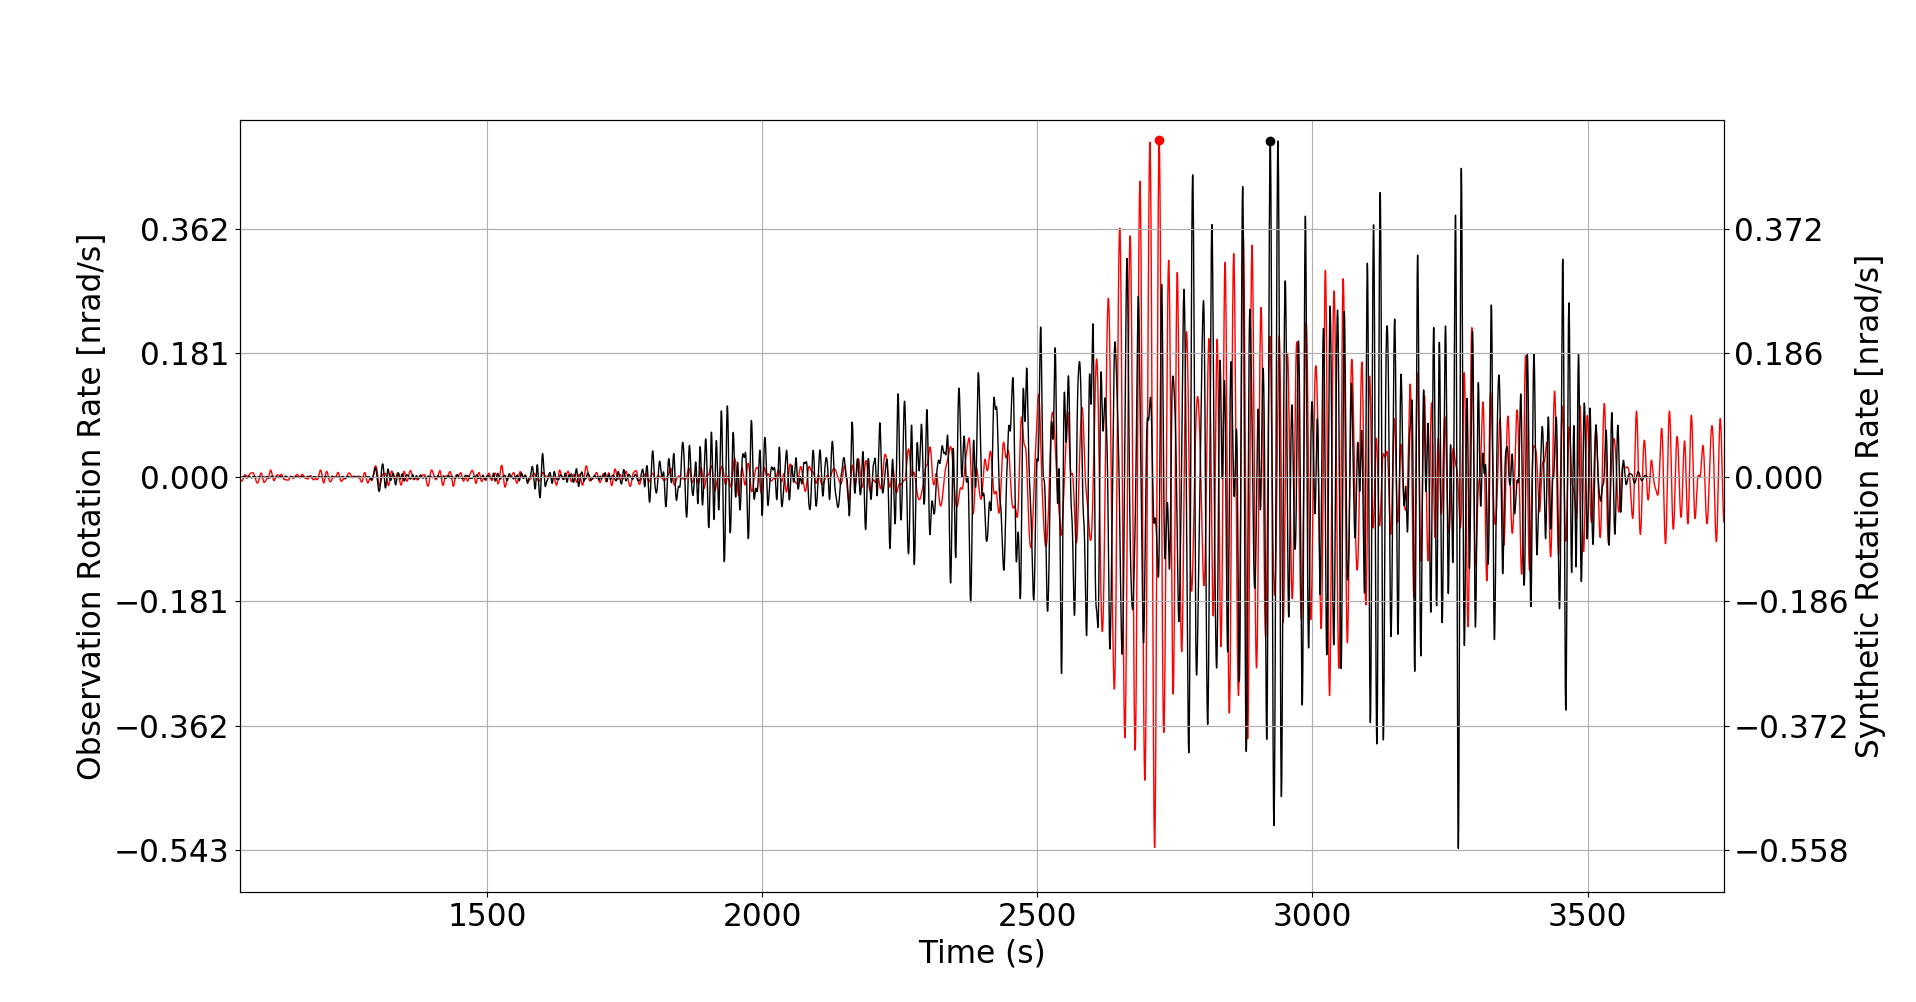
\includegraphics[width=0.5\textwidth]{C201304191958A_10-60_rotationrate_compare}}
\caption{A comparison of synthetic and observed waveforms for an M6.1 event, East of Kuril Islands. Waveforms filtered at dominant period 20s.}
\label{fig:both}
\end{figure}

% stopped here
\subsection{Synthetic magnitude scales}
Results derived from synthetic seismograms, shown in Table \ref{tab:scales}, vary quite dramatically from the observed results; these results do not reflect the same discrepancies that are present in the values given by observations.

A visual representation for the synthetic rotation rate magnitude scale $M_{RR}^{SYN}$ is shown in Figure \ref{fig:syn_scale}. The distribution of points on this scale is much more uniform compared to \ref{fig:syn_obs}, which can be attributed to the increased number of recordings for a single event due to the large number of synthetic stations. With so many station receiver pairs over a range of epicentral distances, there are roughly six times more observation points, which provides stronger coverage of epicentral distances. The number of events at very close distances is also quite low, similarly due to the imposed geographic considerations. The 95\% confidence intervals provide a much narrower band, due to the larger number of events and the synthetic nature of this scale; single events providing data points over the entire distance range puts a strong constraint on the fitted decay constants.
%look at equation for confidence interval, what controls it

The synthetic magnitude scales all exhibit very similar values for the decay constant B. The large variation in decay as seen in the observations is not captured here. Compared to the IASPEI magnitude scale, all the synthetic scales fall much lower in their value of B. Synthetic rotation rate gives the largest, or steepest decay constant at 1.215, by only a small margin. Transverse velocity falls in with the smallest value. Looking at the values of C, expected amplitudes are all also quite high, except for rotation rate. Vertical velocity exhibits a n

\begin{figure*}
\centerline{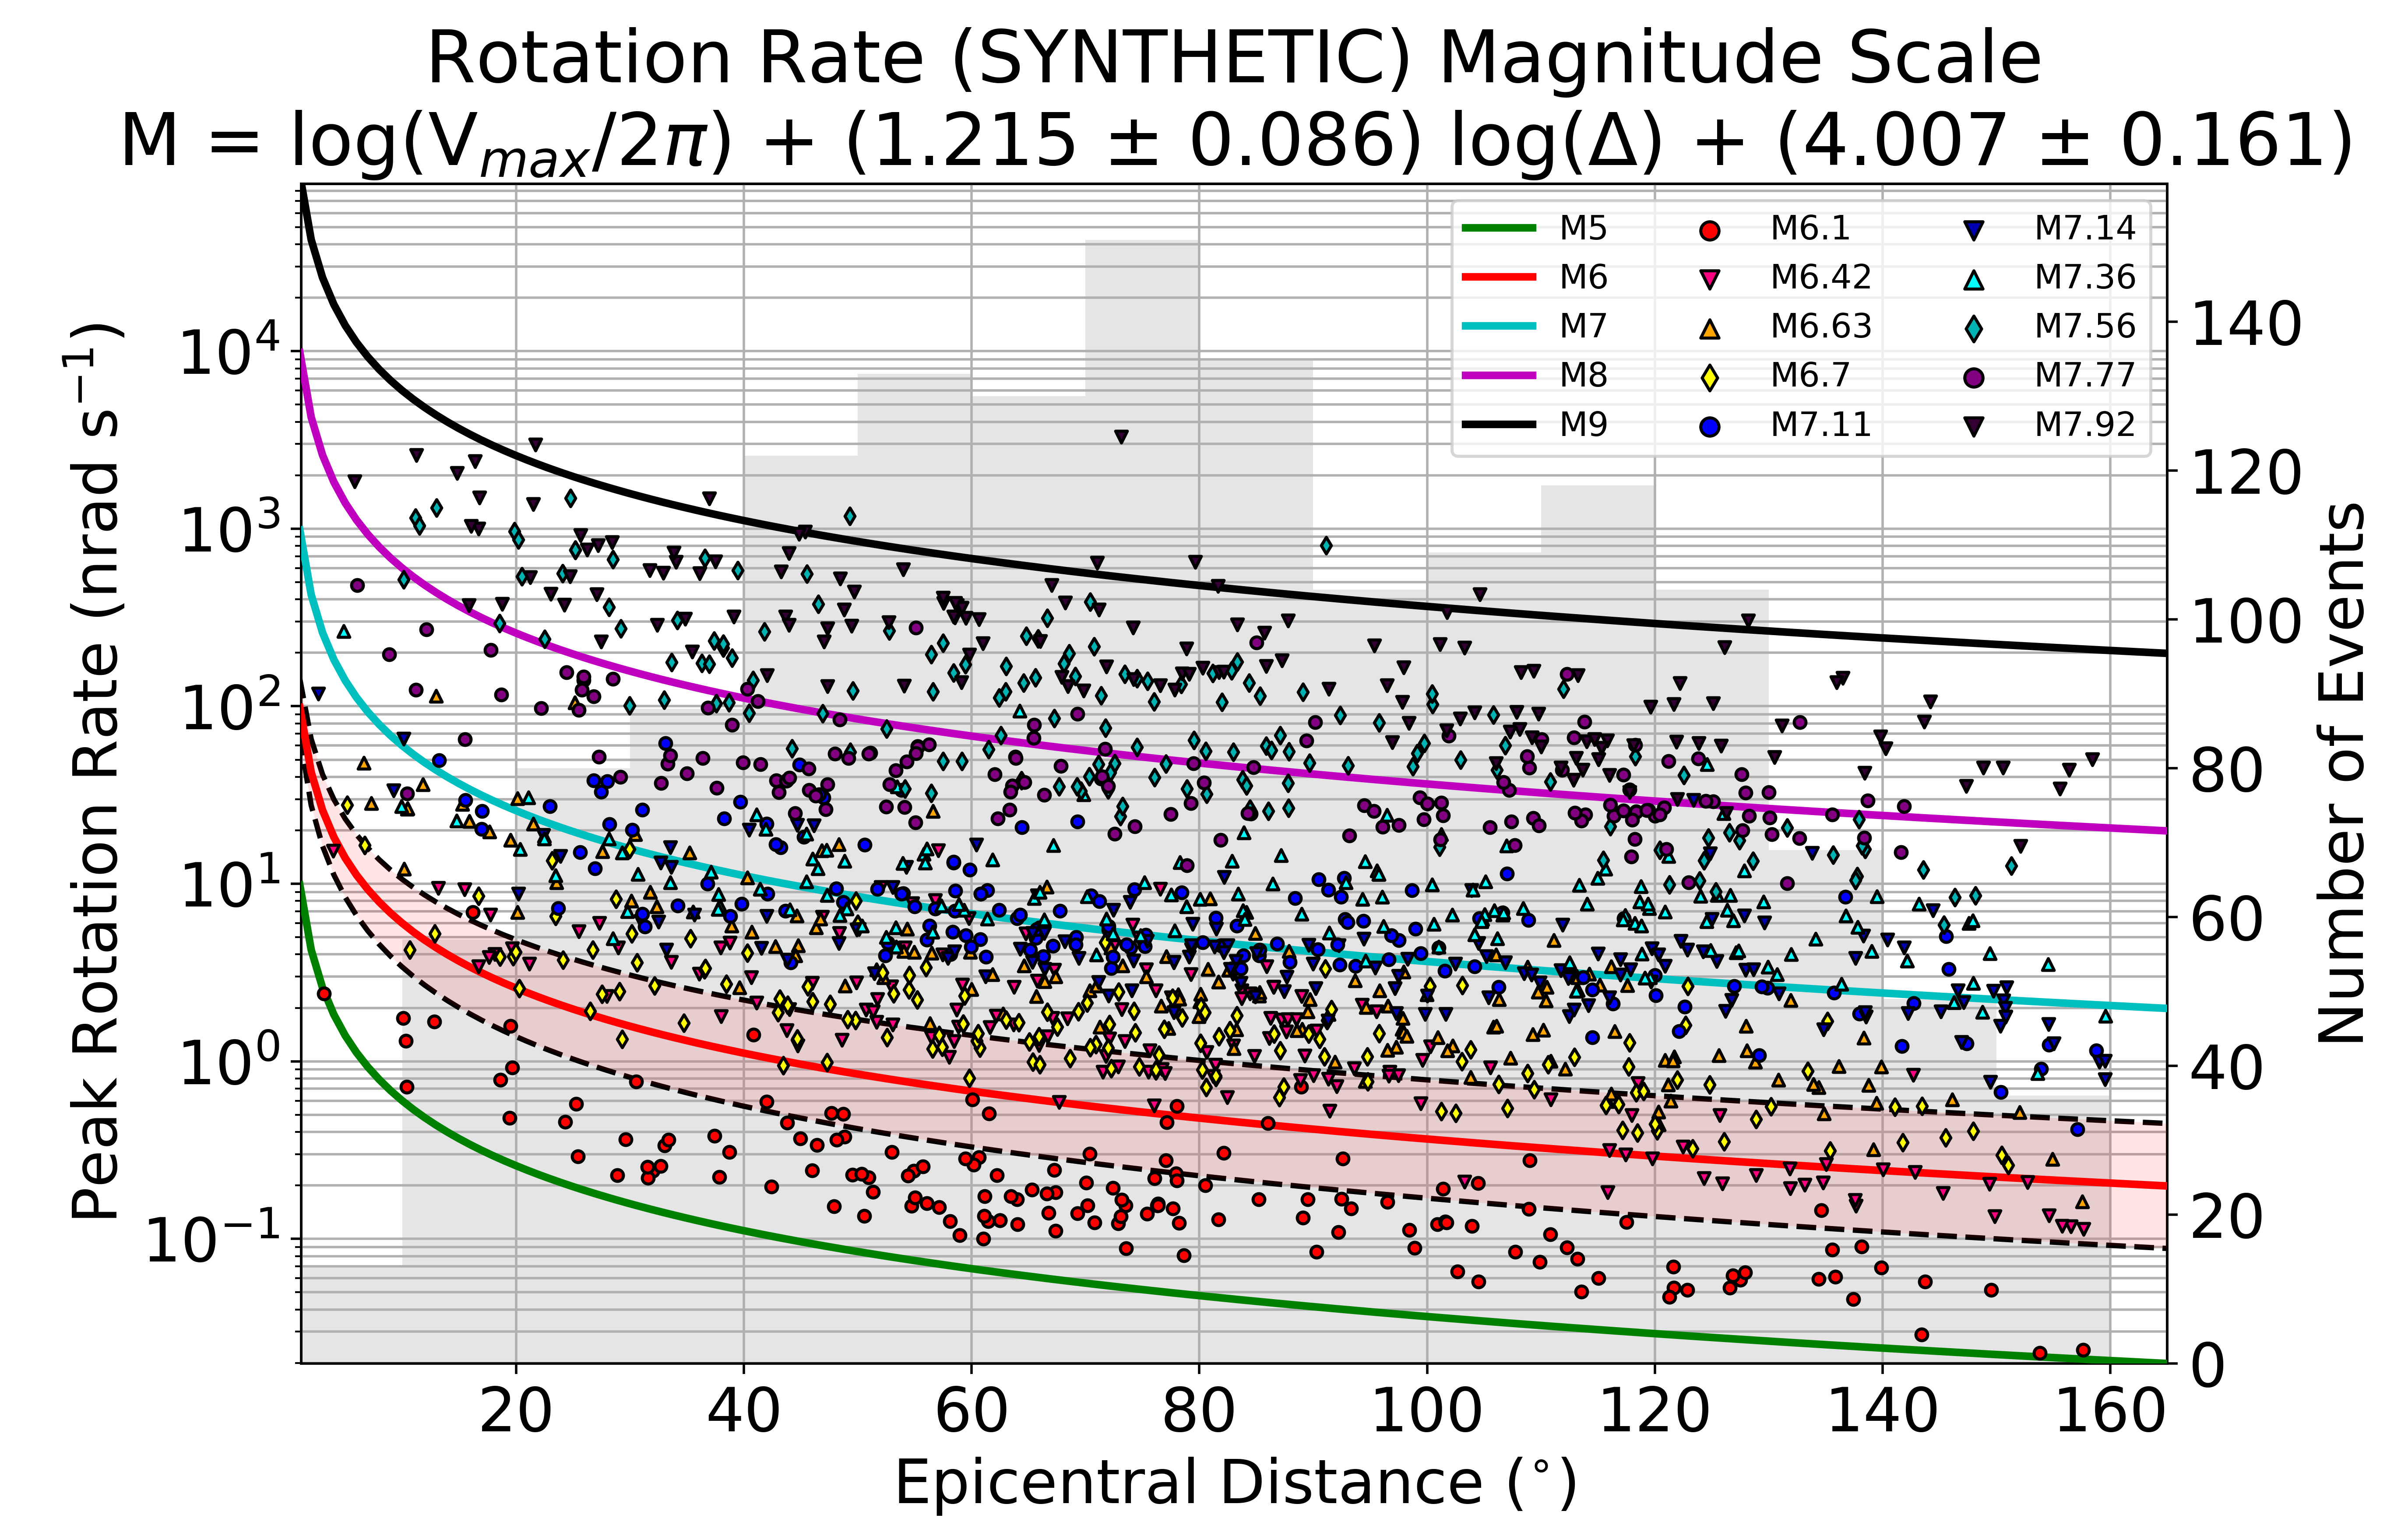
\includegraphics[width=0.8\textwidth]{RR_SYN}}
\caption{Rotation rate magnitude scale for synthetics. All objects similarly represented as in Figure \ref{fig:rr_obs}. Colors of points here represent individual events simulated (for event information, see Table \ref{tab:syn_events}).}
\label{fig:syn_scale}
\end{figure*}

\begin{table*}
\begin{minipage}{115mm}
	\begin{center}
		\begin{tabular}{ |l|c|c|c|c| } 
		        \bf{Scale} & \bf{Label} & \bf{B} & \bf{C}  & \bf{Wave}\\ \hline
        IASPEI & $M_{S}^{BB}$ & 1.66 & 0.3  & Rayleigh \\ \hline
        Herak Herak 1993 & $M_{S}^{HH}$ & 1.094 & 1.429  & Rayleigh \\ \hline
        Ambraseys-Free 1997 & $M_{S}^{AF}$ & 0.947 & 1.77  & Rayleigh \\ \hline
        Rotation  & $M^{RLAS}_{RT}$ & 1.557 $\pm$ 0.295 & 4.186 $\pm$ 0.569  & Love \\ \hline
        Rotation Rate & $M^{RLAS}_{RR}$ & 1.823 $\pm$ 0.303 & 4.113 $\pm$ 0.586  & Love\\ \hline 
        Transverse Velocity (Wettzell) & $M^{WET}_T$ & 1.45 $\pm$ 0.27 & 0.527 $\pm$ 0.521 & Love \\ \hline
        Transverse Velocity (FFB) & $M^{FUR}_T$ & 1.442 $\pm$ 0.27 & 0.447 $\pm$ 0.523 & Love \\ \hline
        Vertical Velocity (Wettzell) & $M^{WET}_Z$ & 1.084 $\pm$ 0.264 & 1.093 $\pm$ 0.511  & Rayleigh \\ \hline
        Vertical Velocity (FFB) & $M^{FUR}_Z$ & 1.095 $\pm$ 0.259 & 1.09 $\pm$ 0.502  & Rayleigh \\ \hline
		\end{tabular}
		
    		\caption{Magnitude scales and derived constants with 95\% confidence intervals for observations at instruments RLAS, WET (Wettzell, Germany) and FUR (F\"urstenfeldbruck, Germany), for equations of the form $M = log_{10}(V/2\pi) + B\cdot log_{10}(\Delta) + C$. The final column gives consideration to the wave type that each instrument component should provide a proxy for.}
		\label{tab:scales}
	\end{center}
	\end{minipage}
\end{table*}

\begin{table*}
\begin{minipage}{115mm}
	\begin{center}
		\begin{tabular}{ |l|c|c|c|c| } 
		        \bf{Scale} & \bf{Label} & \bf{B} & \bf{C}  & \bf{Wave}\\ \hline
        Synthetic Rotation  & $M^{SYN}_{RT}$ & 1.204 $\pm$ 0.086 & 3.841 $\pm$ 0.159  & Love \\ \hline
	Synthetic Rotation Rate & $M^{SYN}_{RR}$ & 1.215 $\pm$ 0.086 & 4.007 $\pm$ 0.161  & Love\\ \hline 
        Synthetic Transverse Velocity & $M^{SYN}_T$ & 1.094 $\pm$ 0.081 & 0.146 $\pm$ 0.16 & Love \\ \hline
        Synthetic Vertical Velocity  & $M^{SYN}_Z$ & 1.206 $\pm$ 0.08 & -0.011 $\pm$ 0.149  & Rayleigh \\ \hline
		\end{tabular}
		
    		\caption{Synthetic magnitude scales and derived constants with 95\% confidence intervals, for equations of the form $M = log_{10}(V/2\pi) + B\cdot log_{10}(\Delta) + C$. The final column gives consideration to the wave type that each instrument component should provide a proxy for.}
		\label{tab:syn_scales}
	\end{center}
	\end{minipage}
\end{table*}


\subsection{Expected rotation amplitudes}
One useful aspect of magnitude scales is to provide an expected amplitude value for a given magnitude event at certain distance. 
%This is quite helpful in areas such as seismic hazard, where one can estimate the order of magnitude of ground motion at a location some distance away from an event, given a certain event size, though this is also dependent on many factors, such as site effects, travel paths, and amplitude modulation due to attenuation, focusing etc. This has largely been replaced by the concept of ground motion prediction equations, however it still provides a useful insight.% something about GMPA

One area of interest in rotational seismology is the development of field deployable sensors. Due to the very low order of magnitudes of rotation signals (measured in nanoradian scale), it is a concern whether or not newly developed field deployable rotation sensors can reach the sensitivity necessary to capture the rotational motion amplitudes excited by regional or tele- seismic events. With the rotational magnitude scale derived here, we are able to create a list of observation based expected amplitudes. At the time of writing, the field deployable rotation sensor BlueSeis from the company iXBlue, has a noise floor of roughly 1 nrad/s/$\sqrt{Hz}$ [Cite iXBlue]. Referring to Table \ref{tab:scales}, the approximate maximum distance the sensor can be placed to detect a M$_w$5 event would be 21$^\circ$ epicentral distance, roughly 2300 km. This distance range would mean current day sensors could detect regional >M5 earthquakes. Other considerations must be taken into account before these values can be used for field deployment decisions, however it provides a useful jumping off point for future instrument deployments.

%smallest events discernible on observatory based rlas?


\section{Discussion}
% motivation for the work
The long term continuous recordings of rotation and translation waveforms at Wettzell has provided us an extensive catalog of colocated observations to explore seismic signals of events with largely varying source parameters and travel paths. The motivation for addressing amplitude decays in the initial study of Igel et al. 2007, was to determine whether or not decay of peak observed rotation rates was consistent with the definition of the commonly used surface wave magnitude equation. In this study we expanded our motivation to include the comparison of decay rates between rotations and translations, to see if and how these quantities might differ. Measurements of seismically induced rotation amplitudes have never been addressed on such a scale, and  if rotations are to someday be incorporated into standard seismological practices, it is useful and beneficial to understand the general characteristics of their observed signals.

%discussion of results
The rotation based magnitude scales presented in Table \ref{tab:scales} present the idea that rotation amplitude decay is not exceedingly different from those for translation measurements; that is, values of B are not orders of magnitude different. Since rotation measurements in the surface wave train sample the horizontal nature of the Love wave, this finding is not so surprising, and of course was already shown previously by Igel et al. 2007. It does prove reassuring that instruments measuring rotation, given the necessary resolution, will not face any differences in recording events at distance.

Although translation measurements exhibit lower values of B, it has been stated previously (Herak/Ambraseys) that this result is not unexpected, and perhaps even a better representation of the surface wave amplitude decay. The stark contrast between the values of B for scales sensitive to Love waves versus Rayleigh waves is very interesting. Taking theoretical assumptions into account, we can use these results to make the statement that Love waves have a faster amplitude decay rate  compared with  Rayleigh waves. This statement is of course through instrumental proxies, however we can strengthen the case by taking transverse velocity into consideration, which has a value of B that lies closer to that of rotation (because we are using the same events for all scales considered, we are confident that these comparisons are made fairly); determining transverse velocity is dependent on correct rotating the North and East components, and it is possible that incorrect rotation can lead to mixing of Love waves and the radial component of Rayleigh waves. If radial and vertical components of Rayleigh waves decay at the same rate, then this would lead to the effect seen in Table \ref{tab:scales}: a slightly lower value of B than that of rotation, a scale that is instrumentally insensitive to translations. (A backazimuth value that is incorrect by 10$^\circ$ changes the expected amplitude of the transverse component by 75\%.) %where to add this?

Although moment magnitude has proven a more grounded measure of earthquake size, surface wave magnitude is still used by agencies around the world. Previous literature has recommended that this scale should be amended in the face of having a potential distance bias. In this study we report the same findings: the current values of B and C for the surface wave magnitude scale are insufficient in predicting the magnitude based on surface wave amplitude values; both observationally and synthetically we show that values of B are systematically lower than the current value of B = 1.66.

Synthetic results prove drastically different from those predicted by observations, and warrants the doubt whether our synthetics lack the detail necessary to fully capture the reality of earth structure which strongly affects amplitudes of surface waves. 3D crust and mantel models, including topography and a host of other factors that play a role in surface wave amplitudes, still predicted amplitudes one order of magnitude larger than those observed at our stations. This large discrepancy points to a need for a more detailed and realistic full earth model than what is available at the time of writing, if it is to be used for this purpose of determining amplitude decays.

%questions that arise from the results
Many questions arose from analysis of these results which would prove interesting to investigate, but fall outside the scope of this paper. One such question is understanding the cause of discrepancy between observed rotation and translation amplitude decays. If this is a detail related to the observable, would this affect still be seen if these analyses were also performed on rotation derived through array methods, or is this effect only noticeable on instruments operating on Sagnac interferometry. If, rather, this effect is a factor of the wavetypes our instruments are sensitive to: what, theoretically, causes the difference in decay rates between Love waves and Rayleigh waves? Is this detectable in other regions and tectonic settings, or only seen for stations on the European continent? Perhaps this magnitude scale analysis could be performed only for tranvserse, radial and vertical components of single stations, to see if these values of B and C are recovered in other areas. In regards to the synthetics, what sort of modifications to our earth models are required to reproduce the effects we are seeing with our observations? If point sources are insufficient in producing the teleseismic amplitudes we observe, what level of complexity is required to accurately model waves at these periods and distances? In the same vein, how important is the observation setup; does number of stations, receivers and station-receiver pairs have a strong impact on the values we recover? Would an observational setup with hundreds of sensors and events provide a different perspective than what we have seen here? Finally in regards to a rotation based magnitude scale; if we are observing such large differences between rotation and vertical velocity based magnitude scales, this might warrant defining a new magnitude scale solely for Love waves. Ground motion from these Love and Rayleigh waves are starkly different and perhaps one single surface wave magnitude scale is insufficient. If these discrepancies show up also in previous literature, perhaps it is necessary to instead define M$_S^{LOVE}$ and M$_S^{RAYLEIGH}$ to replace the current M$_S^{BB}$. At the time of writing, with the push for field deployable rotation sensors and with an increasing number of rotation observations available, it would be possible to quickly determine peak amplitudes of rotations for incoming surface waves and define some magnitude based on an instrument only sensitive to Love waves, extremely useful because it does not require the precise position of the event for determining the correct backazimuth. If this is the case, we propose in this discussion that the current rotation based magnitude scale given in Table \ref{tab:scales} should be used as a preliminary Rotation magnitude scale for determining magnitudes of events for instruments measuring rotation on the vertical axis. We expect further observations, instruments and catalogs will be used to refine these preliminary values.

%future work and suggestions if work is expanded on
A lack of observations at epicentral distances less than 20$^\circ$ and greater than 140$^\circ$ provides large uncertainties in the accuracy of our rotation magnitude scale. Going forward, it would be immensely beneficial to collect peak amplitude values at these distances to provide further constraint on our magnitude scales. The inclusion of more stations recording the same event would also make these derived scales much more robust. Since it may be a some time before full networks of permanent six component stations are available, inclusion of array derived rotations would prove the most useful method in providing more data for determination of these magnitude scales. For synthetics, deeper exploration of individual waveforms might assist in understanding where our current global models fail in accurately recreating real world observations. 
%In deciding how to run our synthetics, ideas were proposed for different combinations of crustal and mantle models, and those effects on the resulting amplitudes. A lack of time never saw this idea come to fruition, however it would have been a very interesting approach.

%closing paragraph
Measurements of rotations and spatial gradients has proven a very interesting theoretical aspect of a field which has become extremely proficient in stable observations of three translational components. With this new observable, we are able to revisit theories proposed decades before with a new perspective. With the development of translational and rotational magnitude scales, we have determined some stark differences in observed amplitude decays between these two observables, and believe we can put forth the idea that Love waves exhibit stronger observed amplitude decays compared to Rayleigh waves, and that perhaps it is necessary to split our current definition of surface wave magnitude into two definitive definitions. Time will tell whether these results hold, as rotation measurements become more readily available and accessible, however it is exciting to see how these might change as a new slew of instruments and observations become available to the field of seismology. 

%to add: 
%-basin amplification of love vs rayleigh waves, transverse component shows on average higher amplitude
%-synthetic stations
%-high frequency attenutation of rotation rate compared to rotation
%-herak and herak newly proposed magnitude scale
%-averaging of earth structure not done here
%-considerations towards using the correct backazimuth
%-confidence interval
%-because of the logarithmic nature of magnitude scales, even differences in the decay constant don't make that much of an impact on the resulting expected amplitudes that one sees 
%-using the same value of c for all rotation, at 80 degrees you get an order of magnitude difference in expected amplitude for synthetic and observed scales
%-because we use Mw and therefore Ms as a controlling parameter in our linear regression, it has a strong effect on the end result for our fitted line
%-large earthquakes being approximated as point sources with boxcar-like source time functions - not capturing the effects of the rupture so we aren't matching wiggle by wiggle. Even then we are consistently over predicting amplitudes 
%
%misc:
%how to convert from old magnitude scales to new - just subtract 3 from C (rewriting of magnitude equation)
%
%+ considerations for observations and synthetics - geographical, data, frequency wise
%+ observation results by themselves
%+ synthetic results by themselves
%+ comparisons of observations and synthetics
%+ questions that arose from the processing
%+ further work


\label{lastpage}


\end{document}


%\begin{figure}[h]
%\centerline{\includegraphics[width=0.8\textwidth]{XYZ}}
%\caption{XYZ}
%\end{figure}
